%% 
%% Copyright 2007-2025 Elsevier Ltd
%% 
%% This file is part of the 'Elsarticle Bundle'.
%% ---------------------------------------------
%% 
%% It may be distributed under the conditions of the LaTeX Project Public
%% License, either version 1.3 of this license or (at your option) any
%% later version.  The latest version of this license is in
%%    http://www.latex-project.org/lppl.txt
%% and version 1.3 or later is part of all distributions of LaTeX
%% version 1999/12/01 or later.
%% 
%% The list of all files belonging to the 'Elsarticle Bundle' is
%% given in the file `manifest.txt'.
%% 
%% Template article for Elsevier's document class `elsarticle'
%% with numbered style bibliographic references
%% SP 2008/03/01
%% $Id: elsarticle-template-num.tex 272 2025-01-09 17:36:26Z rishi $
%%
\documentclass[preprint,12pt]{elsarticle}

%% Use the option review to obtain double line spacing
%% \documentclass[authoryear,preprint,review,12pt]{elsarticle}

%% Use the options 1p,twocolumn; 3p; 3p,twocolumn; 5p; or 5p,twocolumn
%% for a journal layout:
%% \documentclass[final,1p,times]{elsarticle}
%% \documentclass[final,1p,times,twocolumn]{elsarticle}
%% \documentclass[final,3p,times]{elsarticle}
%% \documentclass[final,3p,times,twocolumn]{elsarticle}
%% \documentclass[final,5p,times]{elsarticle}
%% \documentclass[final,5p,times,twocolumn]{elsarticle}

%% For including figures, graphicx.sty has been loaded in
%% elsarticle.cls. If you prefer to use the old commands
%% please give \usepackage{epsfig}

%% The amssymb package provides various useful mathematical symbols
\usepackage{amssymb}
%% The amsmath package provides various useful equation environments.
\usepackage{amsmath}
\usepackage{colortbl}
\usepackage{xcolor}
\usepackage{tikz}
\usepackage{booktabs}
\usepackage{algorithm,algorithmic}
\usepackage{pgfplots}
\usepackage{arydshln}
\usepackage{lmodern}
\usepackage{textcomp}
\usepackage{longtable}
\usepackage{pgfplots}
\pgfplotsset{compat=1.17}
\usetikzlibrary{intersections,pgfplots.fillbetween}
\usepackage{float}
\newcommand{\bbR}{\mathbb{R}}
\newcommand{\bbN}{\mathbb{N}}


%% The amsthm package provides extended theorem environments
%% \usepackage{amsthm}

%% The lineno packages adds line numbers. Start line numbering with
%% \begin{linenumbers}, end it with \end{linenumbers}. Or switch it on
%% for the whole article with \linenumbers.
%% \usepackage{lineno}

\journal{Expert Systems with Applications}

\begin{document}

\begin{frontmatter}

%% Title, authors and addresses

%% use the tnoteref command within \title for footnotes;
%% use the tnotetext command for theassociated footnote;
%% use the fnref command within \author or \affiliation for footnotes;
%% use the fntext command for theassociated footnote;
%% use the corref command within \author for corresponding author footnotes;
%% use the cortext command for theassociated footnote;
%% use the ead command for the email address,
%% and the form \ead[url] for the home page:
%% \title{Title\tnoteref{label1}}
%% \tnotetext[label1]{}
%% \author{Name\corref{cor1}\fnref{label2}}
%% \ead{email address}
%% \ead[url]{home page}
%% \fntext[label2]{}
%% \cortext[cor1]{}
%% \affiliation{organization={},
%%             addressline={},
%%             city={},
%%             postcode={},
%%             state={},
%%             country={}}
%% \fntext[label3]{}

\title{ESCaLE: A efficient Personalized Edge Sleep Health Analysis via }

%% use optional labels to link authors explicitly to addresses:
%% \author[label1,label2]{}
%% \affiliation[label1]{organization={},
%%             addressline={},
%%             city={},
%%             postcode={},
%%             state={},
%%             country={}}
%%
%% \affiliation[label2]{organization={},
%%             addressline={},
%%             city={},
%%             postcode={},
%%             state={},
%%             country={}}

\author[label1]{Huimin Zheng}\ead{202210182130@mail.scut.edu.cn} %% Author name
\author[label1]{Xiaofen Xing}\ead{Xfxing@scut.edu.cn} %% Author name
\author[label2]{Xingxing Ai}\ead{cecilialia@stu2023.jnu.edu.cn} %% Author 
\author[label3]{Xueyan Liu}\ead{liuxueyan2010@jnu.edu.cn} %% Author name
\author[label1]{Xiangmin Xu\corref{cor1}}\ead{xmxu@scut.edu.com} %% Author name



%% Author affiliation
\affiliation[label1]{organization={The School of Electronic and Information Engineering, South China University of Technology},%Department and Organization
            addressline={Hongsheng Science and Technology Building, Building 30, South China University of Technology, Wushan Road}, 
            city={Guangzhou},
            postcode={510641}, 
            state={Guangdong},
            country={China}}
%% Author affiliation
\affiliation[label2]{organization={The Nursing College, Jinan University},%Department and Organization
            addressline={No. 601. Huangpu Avenue West, Tianhe District}, 
            city={Guangzhou},
            postcode={510630}, 
            state={Guangdong},
            country={China}}
%% Author affiliation
\affiliation[label3]{organization={Department of Endocrinology and Metabolism, The First Affiliated Hospital of Jinan University},%Department and Organization
            addressline={Huangpu Avenue West, Tianhe District }, 
            city={Guangzhou},
            postcode={510630}, 
            state={Guangdong},
            country={China}}
\cortext[cor1]{Corresponding Author.}

%% Abstract
\begin{abstract}
%% Text of abstract
Personalized health management systems leveraging long-term physiological monitoring have emerged as a critical research frontier, particularly for enabling real-time and privacy-preserving inference on edge devices. While large language models (LLMs) demonstrate strong capabilities in this domain, their computational intensity necessitates cloud dependency, a paradigm fundamentally misaligned with the constrained resources of edge hardware. This paper addresses this challenge through an integrated Chain-of-Thought distillation framework comprising two core components: a LoRA-enhanced Mixture-of-Experts module that transfers complex reasoning patterns from LLMs to compact edge-deployable models, and the hybrid real-world and synthetic data integration from diverse sleep patterns, enabling our system to generate high-quality personalized sleep recommendations, manage follow-up queries efficiently, and deliver accurate domain-specific question answering. Experimental results demonstrate that our distilled model achieves performance comparable to state-of-the-art LLMs while operating efficiently on edge devices. 
\end{abstract}



%%Research highlights
\begin{highlights}
\item Combines CoT distillation with a LoRA-based MoE for efficient edge deployment.
\item Introduces a novel hybrid synthetic data generation method using GPT-4o and Gaussian Copula.
\item Supports multi-task learning for sleep report generation and personalized Q\&A.
\item Delivers a compact 0.5B ESCaLE model that rivals state-of-the-art LLMs.
\item Ablation studies confirm the key role of regularization and CoT instructions.
\end{highlights}

%% Keywords
\begin{keyword}
%% keywords here, in the form: keyword \sep keyword

%% PACS codes here, in the form: \PACS code \sep code

%% MSC codes here, in the form: \MSC code \sep code
%% or \MSC[2008] code \sep code (2000 is the default)
Chain-of-Thought (CoT)\sep Mixture of Experts (MoE)\sep Distillation\sep Large language models (LLMs)\sep Sleep
\end{keyword}

\end{frontmatter}

%% Add \usepackage{lineno} before \begin{document} and uncomment 
%% following line to enable line numbers
%% \linenumbers

%% main text
%%

%% Use \section commands to start a section
\section{Introduction}
\label{sec1}
%% Labels are used to cross-reference an item using \ref command.

Large language models (LLMs) such as GPT-4o and Qwen-max have demonstrated remarkable success in personalized health management by generating tailored recommendations and addressing individual user needs \cite{caruccio2024can}, \cite{cao2024spider2}. However, their reliance on cloud-based deployment introduces challenges including high latency, privacy risks, and substantial resource demands, thereby limiting their suitability for in-time, on-device applications \cite{friha2024llm}. In contrast, smaller language models (SLMs) are more amenable to edge deployment yet typically lack the deep reasoning capabilities and domain-specific expertise required for delivering nuanced, context-aware recommendations.

In the context of edge devices, models with a size limit of approximately 7B parameters are typically the upper bound for smooth operation, as larger models are less suitable for such environments. For personalized sleep health applications, our preliminary experiments, using the Qwen series models as an example, demonstrate that LoRA fine-tuning effectively distills the capabilities of larger models. Models with sizes above 1.5B achieve satisfactory performance, while models with 0.5B parameters exhibit significant performance gaps, as shown in Fig. \ref{model_comparison}. Consequently, this study focuses on a 0.5B model and introduces a novel method aimed at bridging the performance gap. Our approach strives to enable the 0.5B model to achieve comparable performance to larger models in personalized sleep health management.
\begin{figure}[h]
\centerline{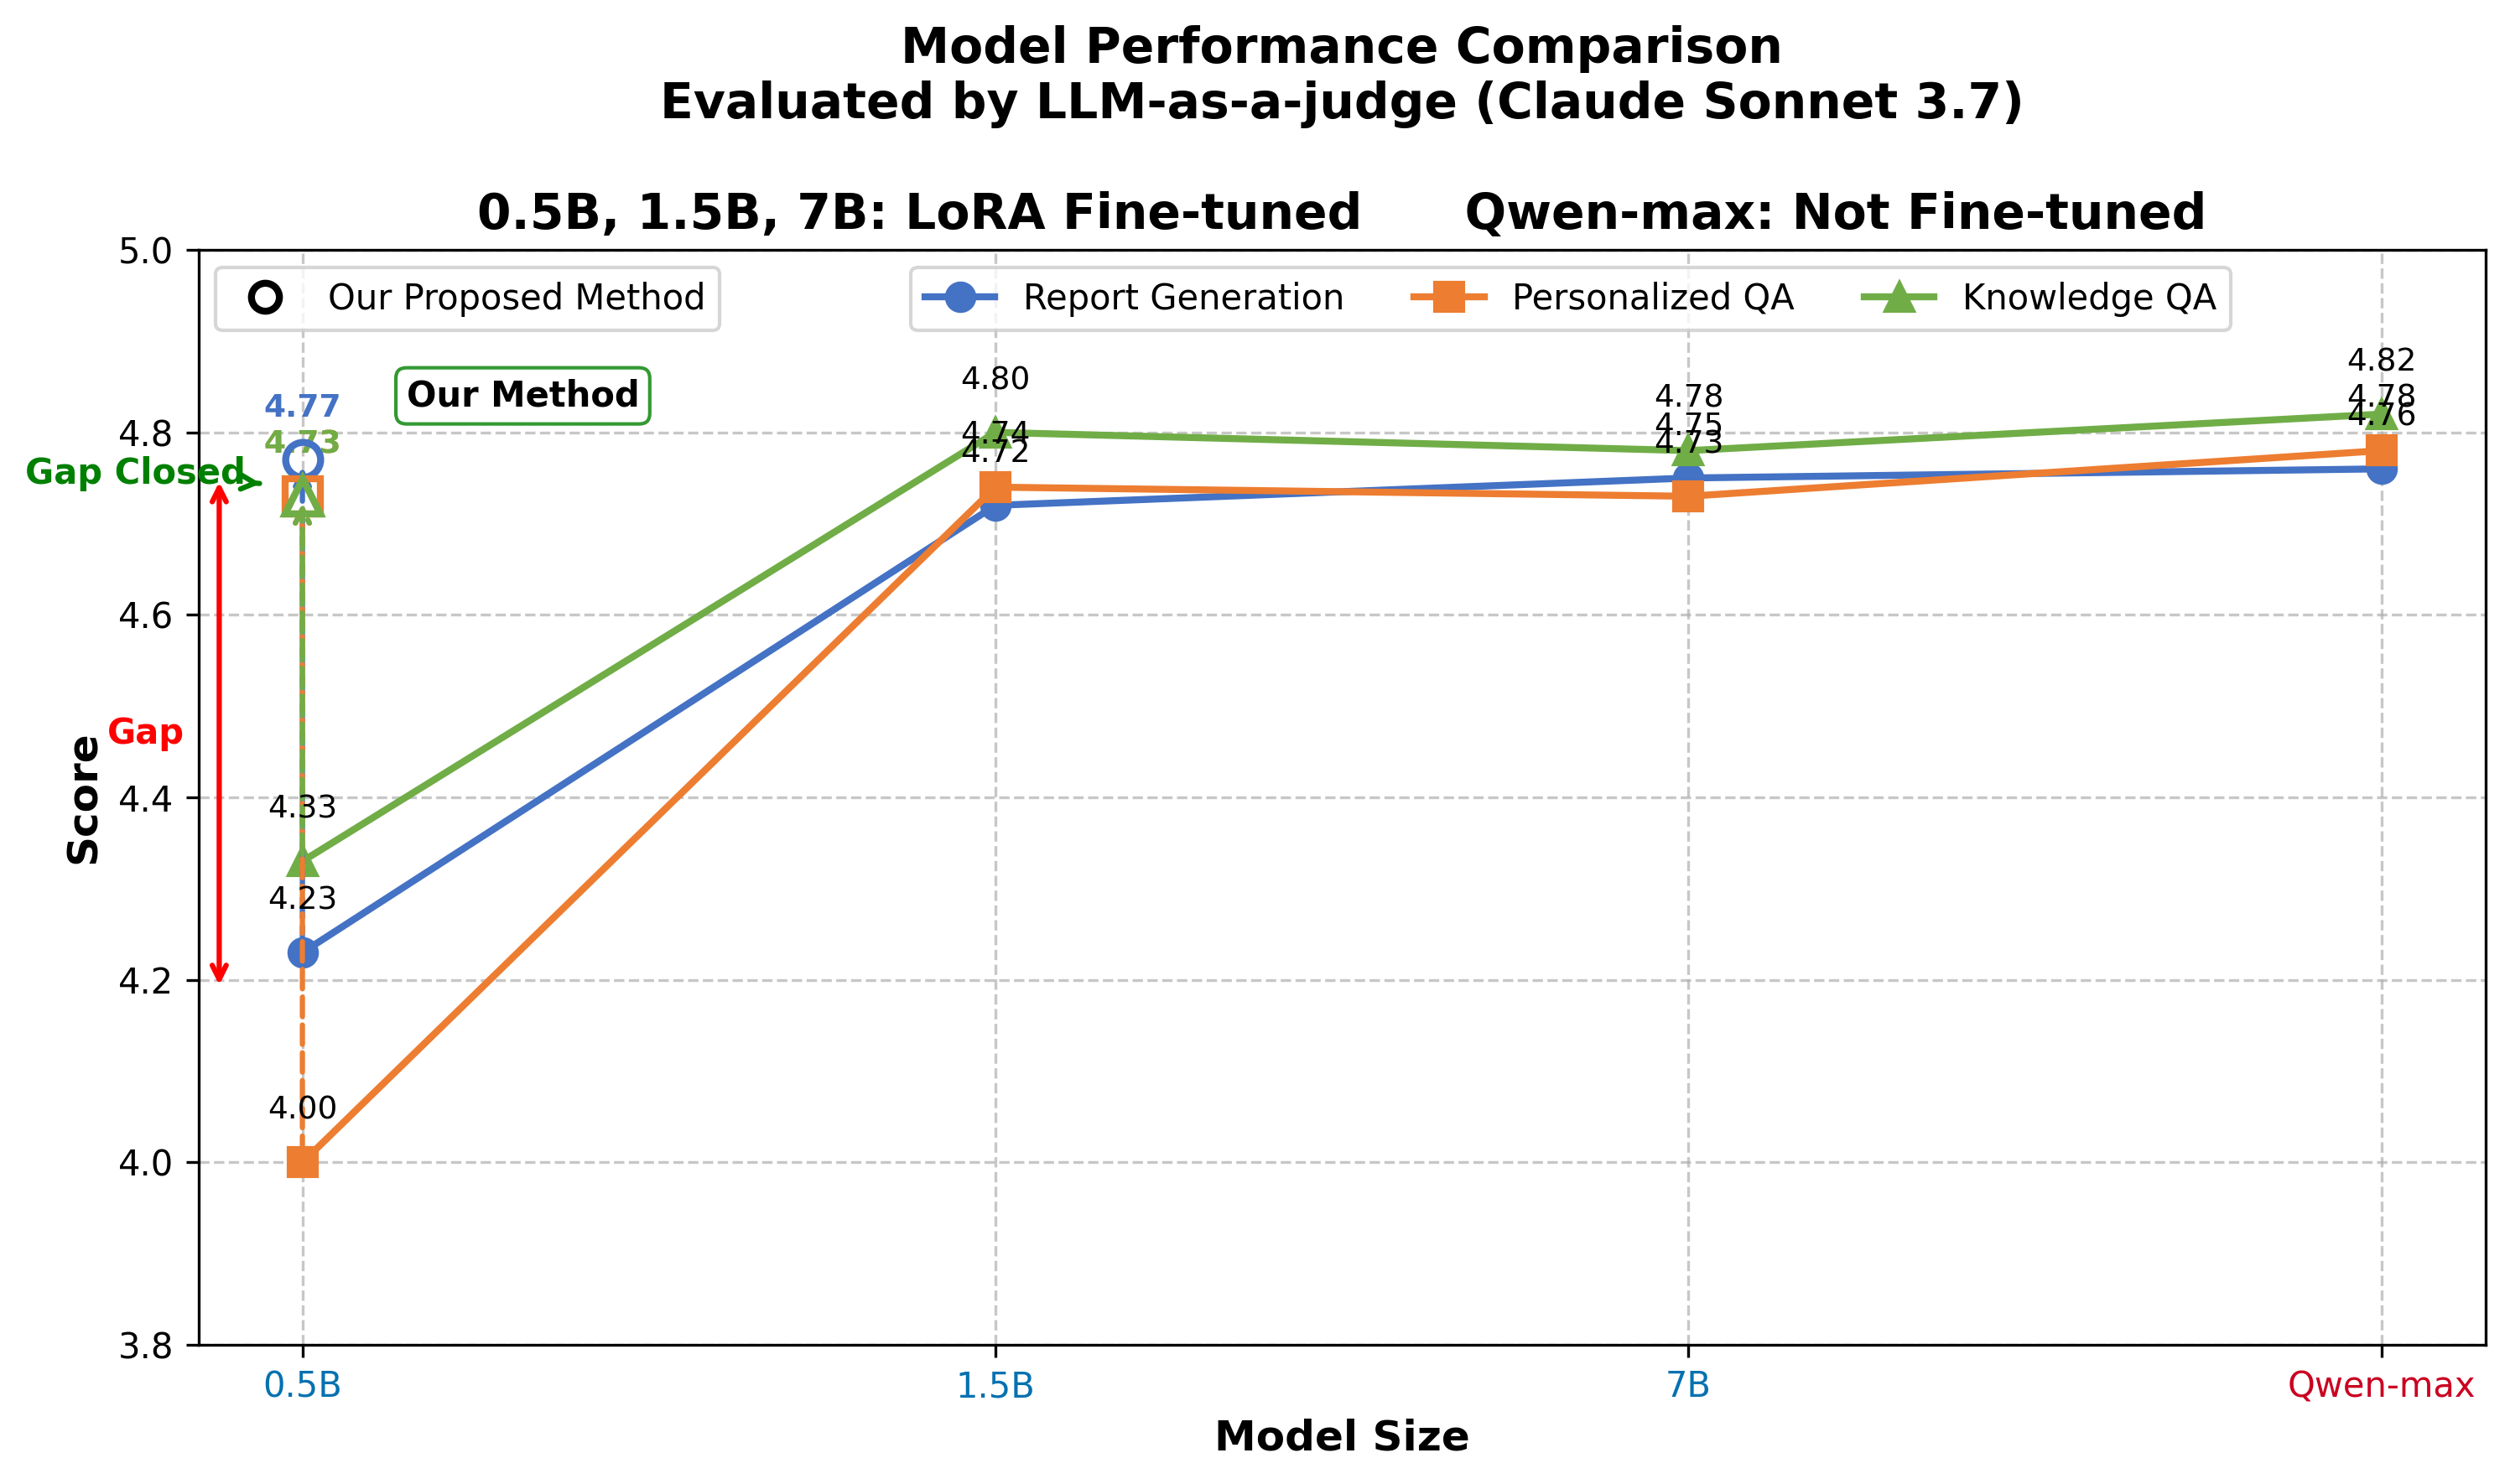
\includegraphics[width=\columnwidth]{model_comparison_line_improved.png}}
\caption{Performance comparison of language models across different parameter sizes for sleep health applications. Models of 0.5B, 1.5B, and 7B were fine-tuned using LoRA, while Qwen-max represents a non-fine-tuned larger model. Evaluation was conducted using LLM-as-a-judge (Claude Sonnet 3.7) across three dimensions: report generation, personalized Q\&A, and knowledge Q\&A. The significant performance gap between the 0.5B model and larger models highlights the challenge addressed in this work: enabling efficient small models (0.5B) that can perform competitively with larger models while remaining deployable on edge devices.}
\label{model_comparison}
\end{figure}


Two primary challenges motivate our work. First, there is limited availability of physiological data, which hampers robust model training \cite{li2025vigilance}. Second, there is a lack of effective multi-task distillation methods tailored specifically for healthcare applications \cite{yang2024survey1}. To address the challenge of physiological data scarcity, we propose a Physiologically-Constrained Adaptive Hierarchical Copula (PC-AHC) method, inspired by Gaussian Copula \cite{merrill2024transforming} and large language model (LLM)-based data synthesis \cite{gan2024towards}. This method is integrated within LLMs to generate synthetic sleep monitoring data that preserves complex interdependencies among parameters while adhering to essential physiological constraints. The PC-AHC framework incorporates constraint-preserving transformations, physiologically-driven copula selection, and cross-system coupling mechanisms to ensure clinical validity. Leveraging the capabilities of LLMs, this approach not only ensures the fidelity of the synthetic data but also enhances its diversity by incorporating information gain, thereby addressing both data scarcity and variability challenges in clinical applications.

Multi-task distillation has been explored using Mixture-of-Experts frameworks in prior work \cite{liu2023moeLoRA, gao2024higher, yang2024moral}, achieving promising results across a range of tasks. Yet, designing MoE architectures that are specifically tailored to healthcare scenarios remains an open research challenge. In this work, we develop a multi-task distillation framework capable of handling tasks such as sleep report generation, personalized question-answering, and domain-specific knowledge question-answering. Our method leverages CoT guidance in combination with LoRA-based MoE instruction fine-tuning to distill advanced reasoning and expert knowledge from state-of-the-art LLMs into the compact ESCaLE model. This approach not only achieves a high degree of personalization but also enables the model to address nuanced user requirements directly on edge devices.
Our contributions can be summarized as follows:
\begin{itemize}
  \item \textbf{Data Synthesis for Enhanced Training}: We propose a novel data synthesis method that integrates GPT-4o with a Gaussian Copula model to generate realistic and diverse sleep datasets. By leveraging statistical distributions and capturing internal correlations, this approach improves data density and representativeness while reducing the need for extensive real-world data collection.
  \item \textbf{Multi-task Learning Framework with CoT and LoRA-based MoE Distillation}: We develop a unified framework that employs Chain-of-Thought distillation alongside a LoRA-based Mixture-of-Experts architecture for multi-task learning. This framework dynamically assigns specialized LoRA adapters to individual tasks, enabling the compact ESCaLE model to inherit advanced reasoning capabilities and domain-specific expertise from large LLMs.
  \item \textbf{Compact and Efficient Sleep Model}: Through rigorous distillation experiments, we demonstrate that our proposed 0.5-billion-parameter ESCaLE model attains performance comparable to state-of-the-art LLMs in tasks such as sleep report generation, personalized question-answering, and domain-specific knowledge question-answering. The optimized design of ESCaLE makes it highly suitable for real-time deployment on resource-constrained edge devices like wearables and smartphones.
\end{itemize}
%% Use \subsection commands to start a subsection.
\section{Related Work}
\subsection{LLM for Wearable Data}
Personal health data from wearable devices are multi-dimensional, continuous, and longitudinal, providing granular insights into individual physiological and behavioral patterns \cite{merrill2024transforming}. Despite its potential, the application of LLMs to wearable health data remains in its infancy, with two main approaches emerging. One preprocesses data (e.g., heart rate, sleep, activity metrics) into features for generating personalized insights. For instance, PH-LLM \cite{cosentino2024towards} fine-tunes Gemini Ultra 1.0 on expert-curated sleep and fitness case studies, using a multimodal adapter to convert wearable sensor data into vectors for personalized recommendations. Similarly, PhysioLLM \cite{fang2024physioLLM} integrates data preparation, GPT-4-based insight generation, and a conversational interface for natural interactions. Unlike large models like GPT-3.5 or Gemini, our work focuses on smaller LLMs (< 2 billion parameters) to optimize computational efficiency, reduce latency, and enable real-time, on-device applications, addressing key challenges in making AI-driven personalized health analysis widely accessible.
\subsection{Data Synthesis}
The limited availability of large-scale, real-world wearable datasets remains a significant challenge in personalized health applications, hindering machine learning models' ability to generalize effectively \cite{merrill2024transforming}. Generative models, such as Variational Autoencoders (VAEs) \cite{kingma2013auto}, Generative Adversarial Networks (GANs) \cite{goodfellow2014generative}, Normalizing Flows \cite{rezende2015variational}, and Diffusion Models \cite{rombach2022high}, have emerged as effective tools for addressing this limitation. By generating synthetic data that closely matches the original data distribution, these models augment training datasets, enhancing model performance, particularly when real data is scarce.
\subsection{LLM Distillation}
Due to resource constraints and real-time requirements \cite{huang2024new}, many studies have focused on distilling LLMs to transfer knowledge \cite{mcdonald2024reducing}, reasoning capabilities \cite{li2024turning}, \cite{kang2024knowledge}, and domain expertise \cite{yuan2024LLM} into smaller, more efficient models. Methods like SOCRATIC CoT \cite{shridhar2022distilling} and KARD \cite{kang2024knowledge} show promise in numerical reasoning and factual judgment but lack the nuanced reasoning needed for personalized health analysis, such as interpreting subtle physiological variations or delivering context-aware recommendations. While CoT techniques \cite{wei2022chain}, \cite{kojima2022large}, \cite{fu2023specializing} focus on step-by-step reasoning, they fall short in addressing the complexities of personalized health scenarios. Recent advancements like MixLoRA \cite{li2024mixlora} and MoRAL \cite{yang2024moral} enable parameter-efficient multi-task fine-tuning but face challenges like overfitting and balancing specialization with generalization.
A concise summary of related work is illustrated in Table \ref{tab:model-comparison}.
\begin{table}[htbp]
\caption{Comparison of different models and their characteristics}
\label{tab:model-comparison}
\centering
\begin{tabular}{|c|c|c|c|c|}
\hline
\rowcolor{gray!20}
Model & Deploy & Synthesis Data & Distillation & Performance. \\
\hline
\rowcolor{pink!20}
PH-LLM & Cloud & 
\includegraphics[height=10pt]{wrong.png} & 
\includegraphics[height=10pt]{wrong.png} & 
\includegraphics[height=10pt]{goods.png} \\
\hline
\rowcolor{pink!20}
PhysioLLM & Cloud & 
\includegraphics[height=10pt]{wrong.png} & 
\includegraphics[height=10pt]{wrong.png} & 
\includegraphics[height=10pt]{goods.png} \\
\hline
\rowcolor{pink!20}
PHIA & Cloud & \includegraphics[height=10pt]{correct.png} & 
\includegraphics[height=10pt]{wrong.png} & 
\includegraphics[height=10pt]{goods.png} \\
\hline
\rowcolor{green!20}
SOCRATIC & Edge & 
\includegraphics[height=10pt]{wrong.png} & \includegraphics[height=10pt]{correct.png} & 
\includegraphics[height=10pt]{soso.png} \\
\hline
\rowcolor{green!20}
KARD & Edge & 
\includegraphics[height=10pt]{wrong.png} & \includegraphics[height=10pt]{correct.png} & 
\includegraphics[height=10pt]{soso.png} \\
\hline
\rowcolor{red!20}
ESCaLE & Edge & 
\includegraphics[height=10pt]{Correct.png} & \includegraphics[height=10pt]{correct.png} & 
\includegraphics[height=10pt]{goods.png} \\
\hline
\end{tabular}
\end{table}
\section{Methodology}
To enable efficient, real-time, on-device personalized sleep health analysis, we propose ESCaLE, a compact model that integrates CoT distillation with a LoRA-based MoE framework. ESCaLE effectively transfers reasoning capabilities and expert sleep-related knowledge from large language models (LLMs) into a smaller, resource-efficient model optimized for edge deployment. Our approach addresses three key challenges: (1) limited real-world data, mitigated through advanced data synthesis; (2) multi-task support, achieved via a unified multi-task learning framework; and (3) efficient distillation of reasoning and domain-specific expertise, facilitated by CoT and LoRA-based MoE techniques.  Fig. \ref{fig5} illustrates the application scenario, showcasing the model’s ability to generate detailed sleep reports, respond to personalized queries, and answer knowledge-based questions on sleep health. An QA example is shown in \ref{appendix: QA examplesss}.
\begin{figure}[h]
\centerline{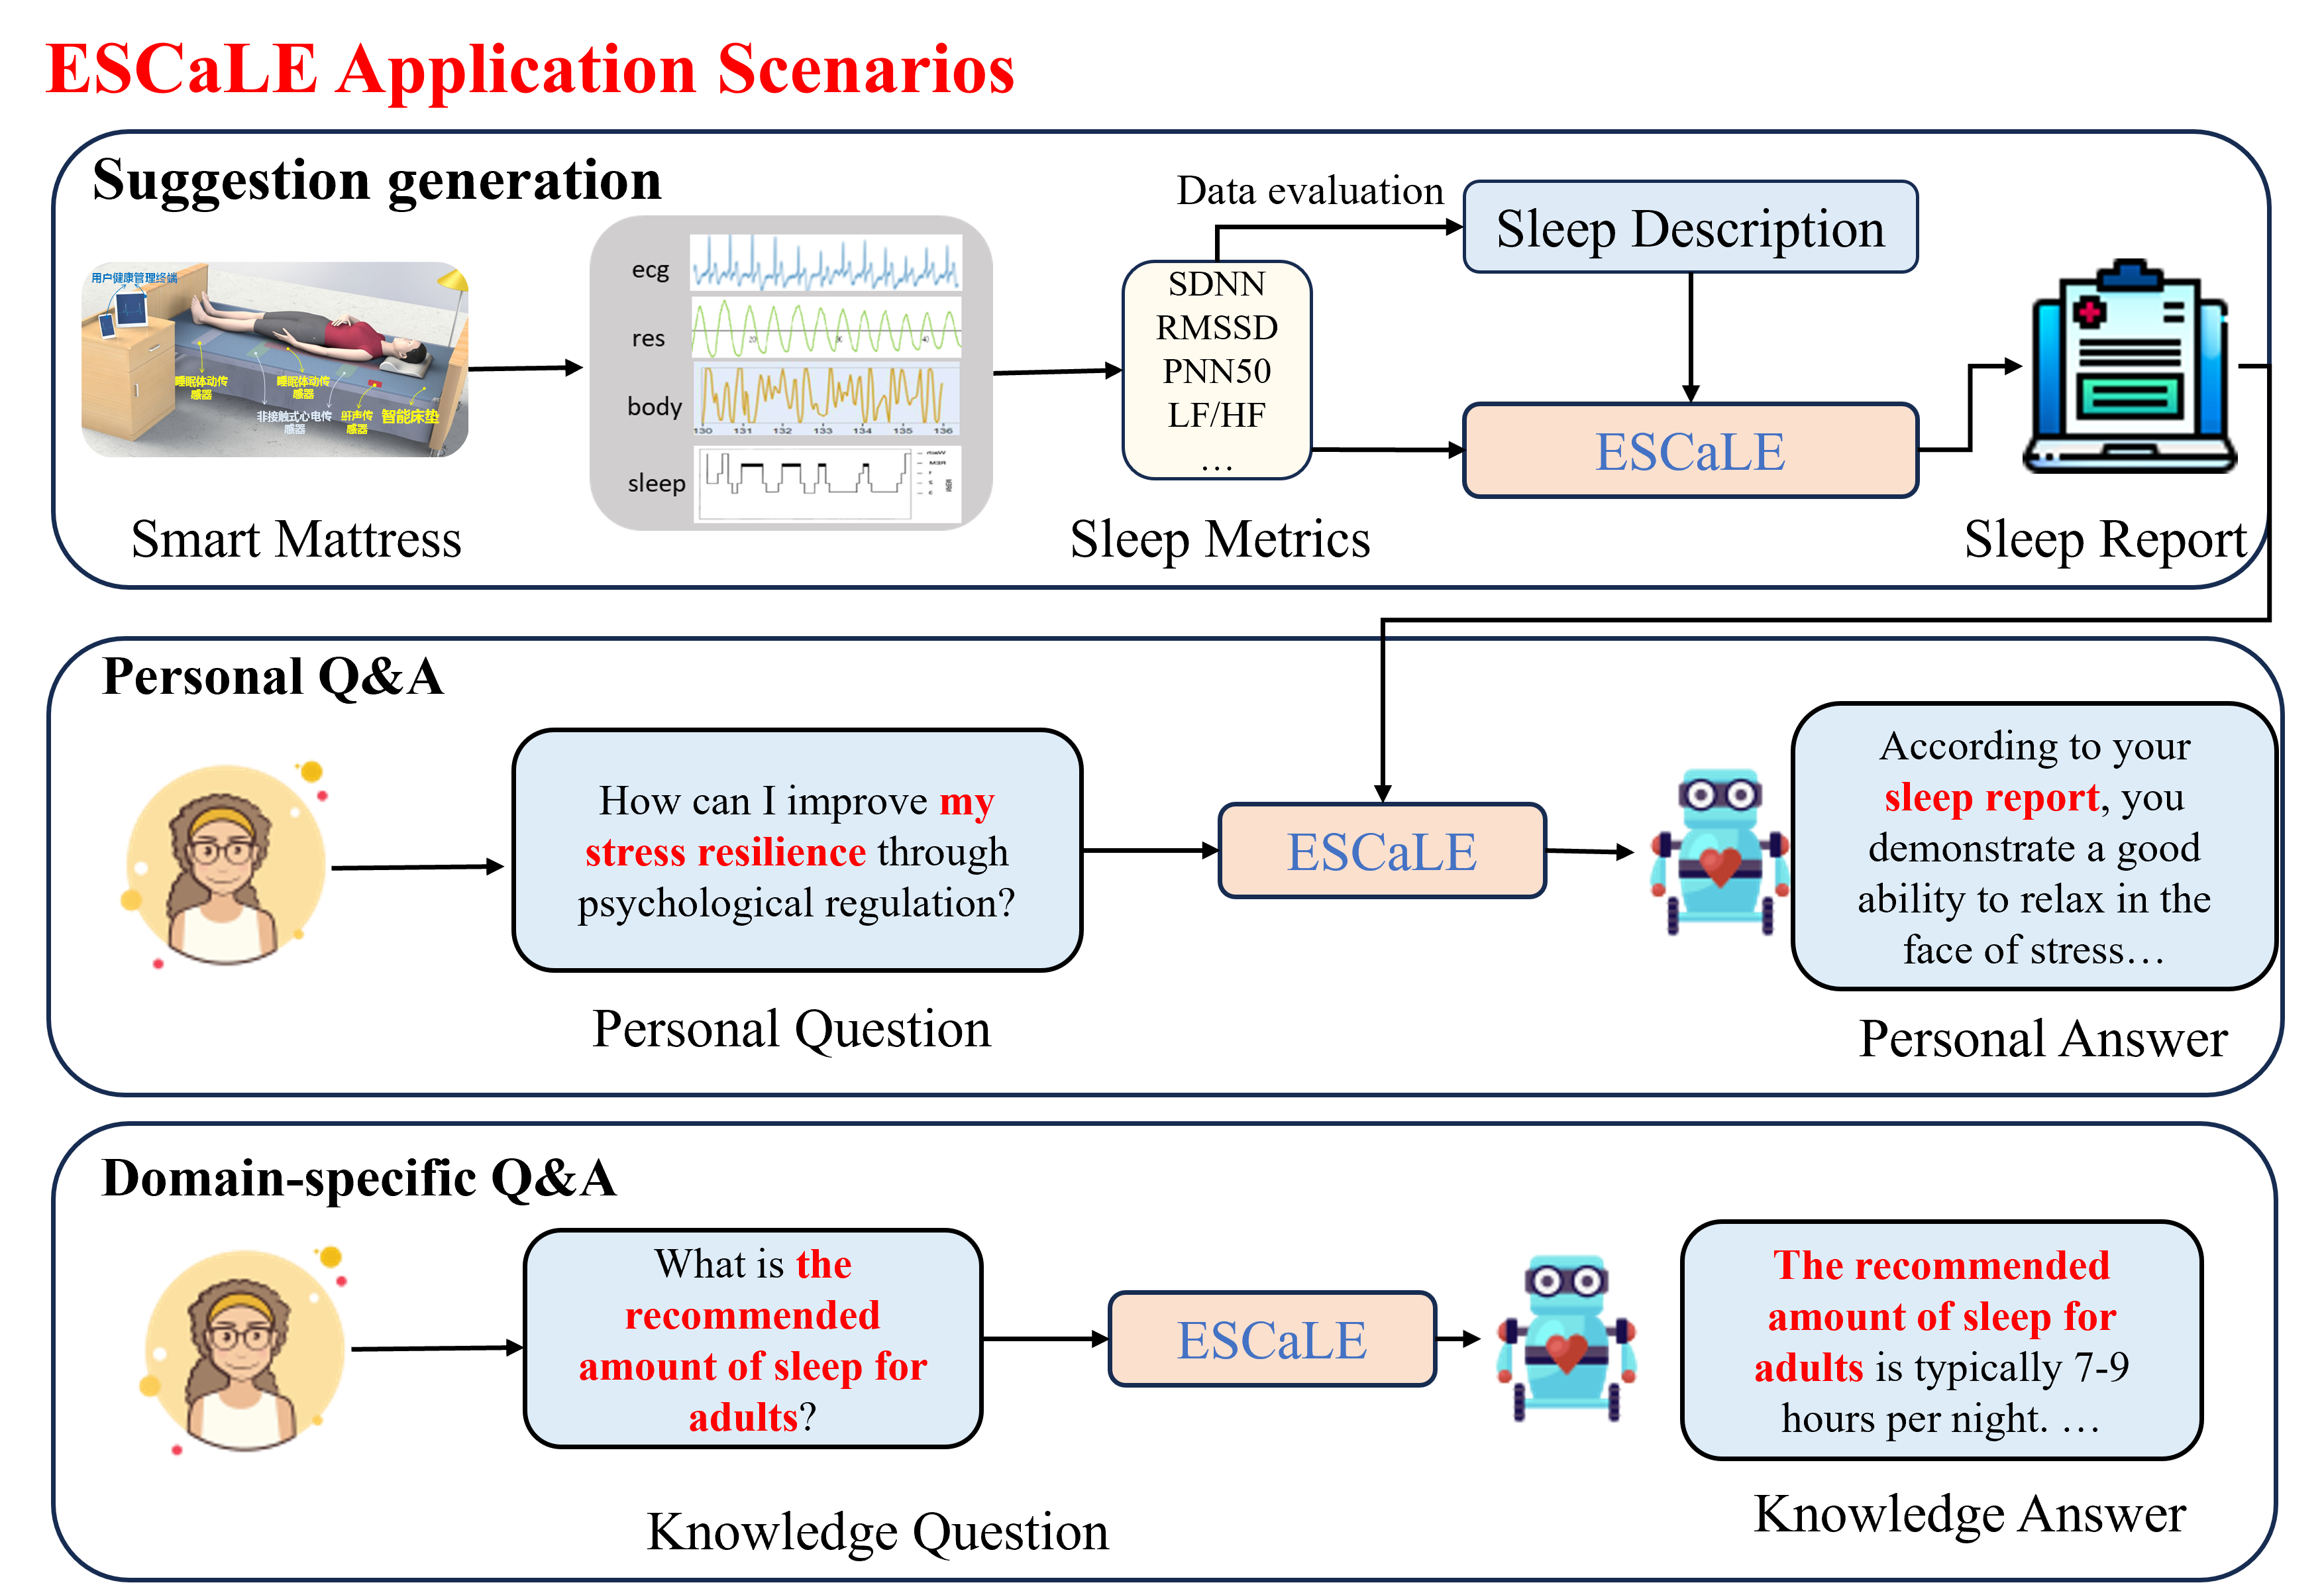
\includegraphics[width=\columnwidth]{applications.png}}
\caption{The ESCaLE Application Scenarios.}
\label{fig5}
\end{figure}

\subsection{Physiologically-Constrained Adaptive Hierarchical Copula with LLM-Guided Optimization}
To address the challenges posed by the limited data volume and diversity in physiological sleep studies, we propose a novel framework, termed \textbf{Physiologically-Constrained Adaptive Hierarchical Copula with Large Language Model Guidance (PC-AHC-LLM)}. This framework integrates hierarchical copula modeling with the physiological reasoning capabilities of large language models (LLMs) to synthesize physiologically consistent sleep parameters. By leveraging the domain knowledge encoded in LLMs, our approach ensures that the generated parameters align with real-world physiological patterns, thereby enhancing the robustness and generalizability of downstream sleep health applications. 

In this study, we focus on seven critical sleep-related parameters, including total sleep duration, deep sleep duration, light sleep duration, and heart rate variability (HRV) features. HRV features, which provide insights into autonomic nervous system activity and sleep quality, were extracted using standard methods to enable a detailed analysis of sleep-related cardiac dynamics. Specifically, we consider the following four key HRV metrics:
\begin{itemize}
    \item \textbf{SDNN (Standard Deviation of NN intervals):} A measure of overall heart rate variability, reflecting the combined influence of sympathetic and parasympathetic nervous system activity.
    \item \textbf{RMSSD (Root Mean Square of Successive Differences):} A metric that captures short-term variations in heart rate, primarily reflecting parasympathetic nervous system activity.
    \item \textbf{LF/HF (Low Frequency/High Frequency ratio):} A ratio representing the balance between sympathetic and parasympathetic nervous system activity, often used to assess autonomic regulation.
    \item \textbf{PNN50 (Percentage of NN intervals greater than 50 ms):} The proportion of adjacent NN intervals differing by more than 50 ms, which serves as an indicator of parasympathetic activity.
\end{itemize}

By synthesizing physiologically consistent sleep parameters, the proposed PC-AHC-LLM framework addresses the limitations of existing datasets and provides a robust foundation for advancing AI-driven sleep health research. The integration of hierarchical copula modeling with LLM-guided physiological reasoning represents a significant step toward generating high-quality, physiologically meaningful data for sleep-related applications.

The PC-AHC-LLM framework comprises two synergistic components (illustrated in Fig.~\ref{PC-AHC-LLM}):
\begin{figure}[t]
\centering
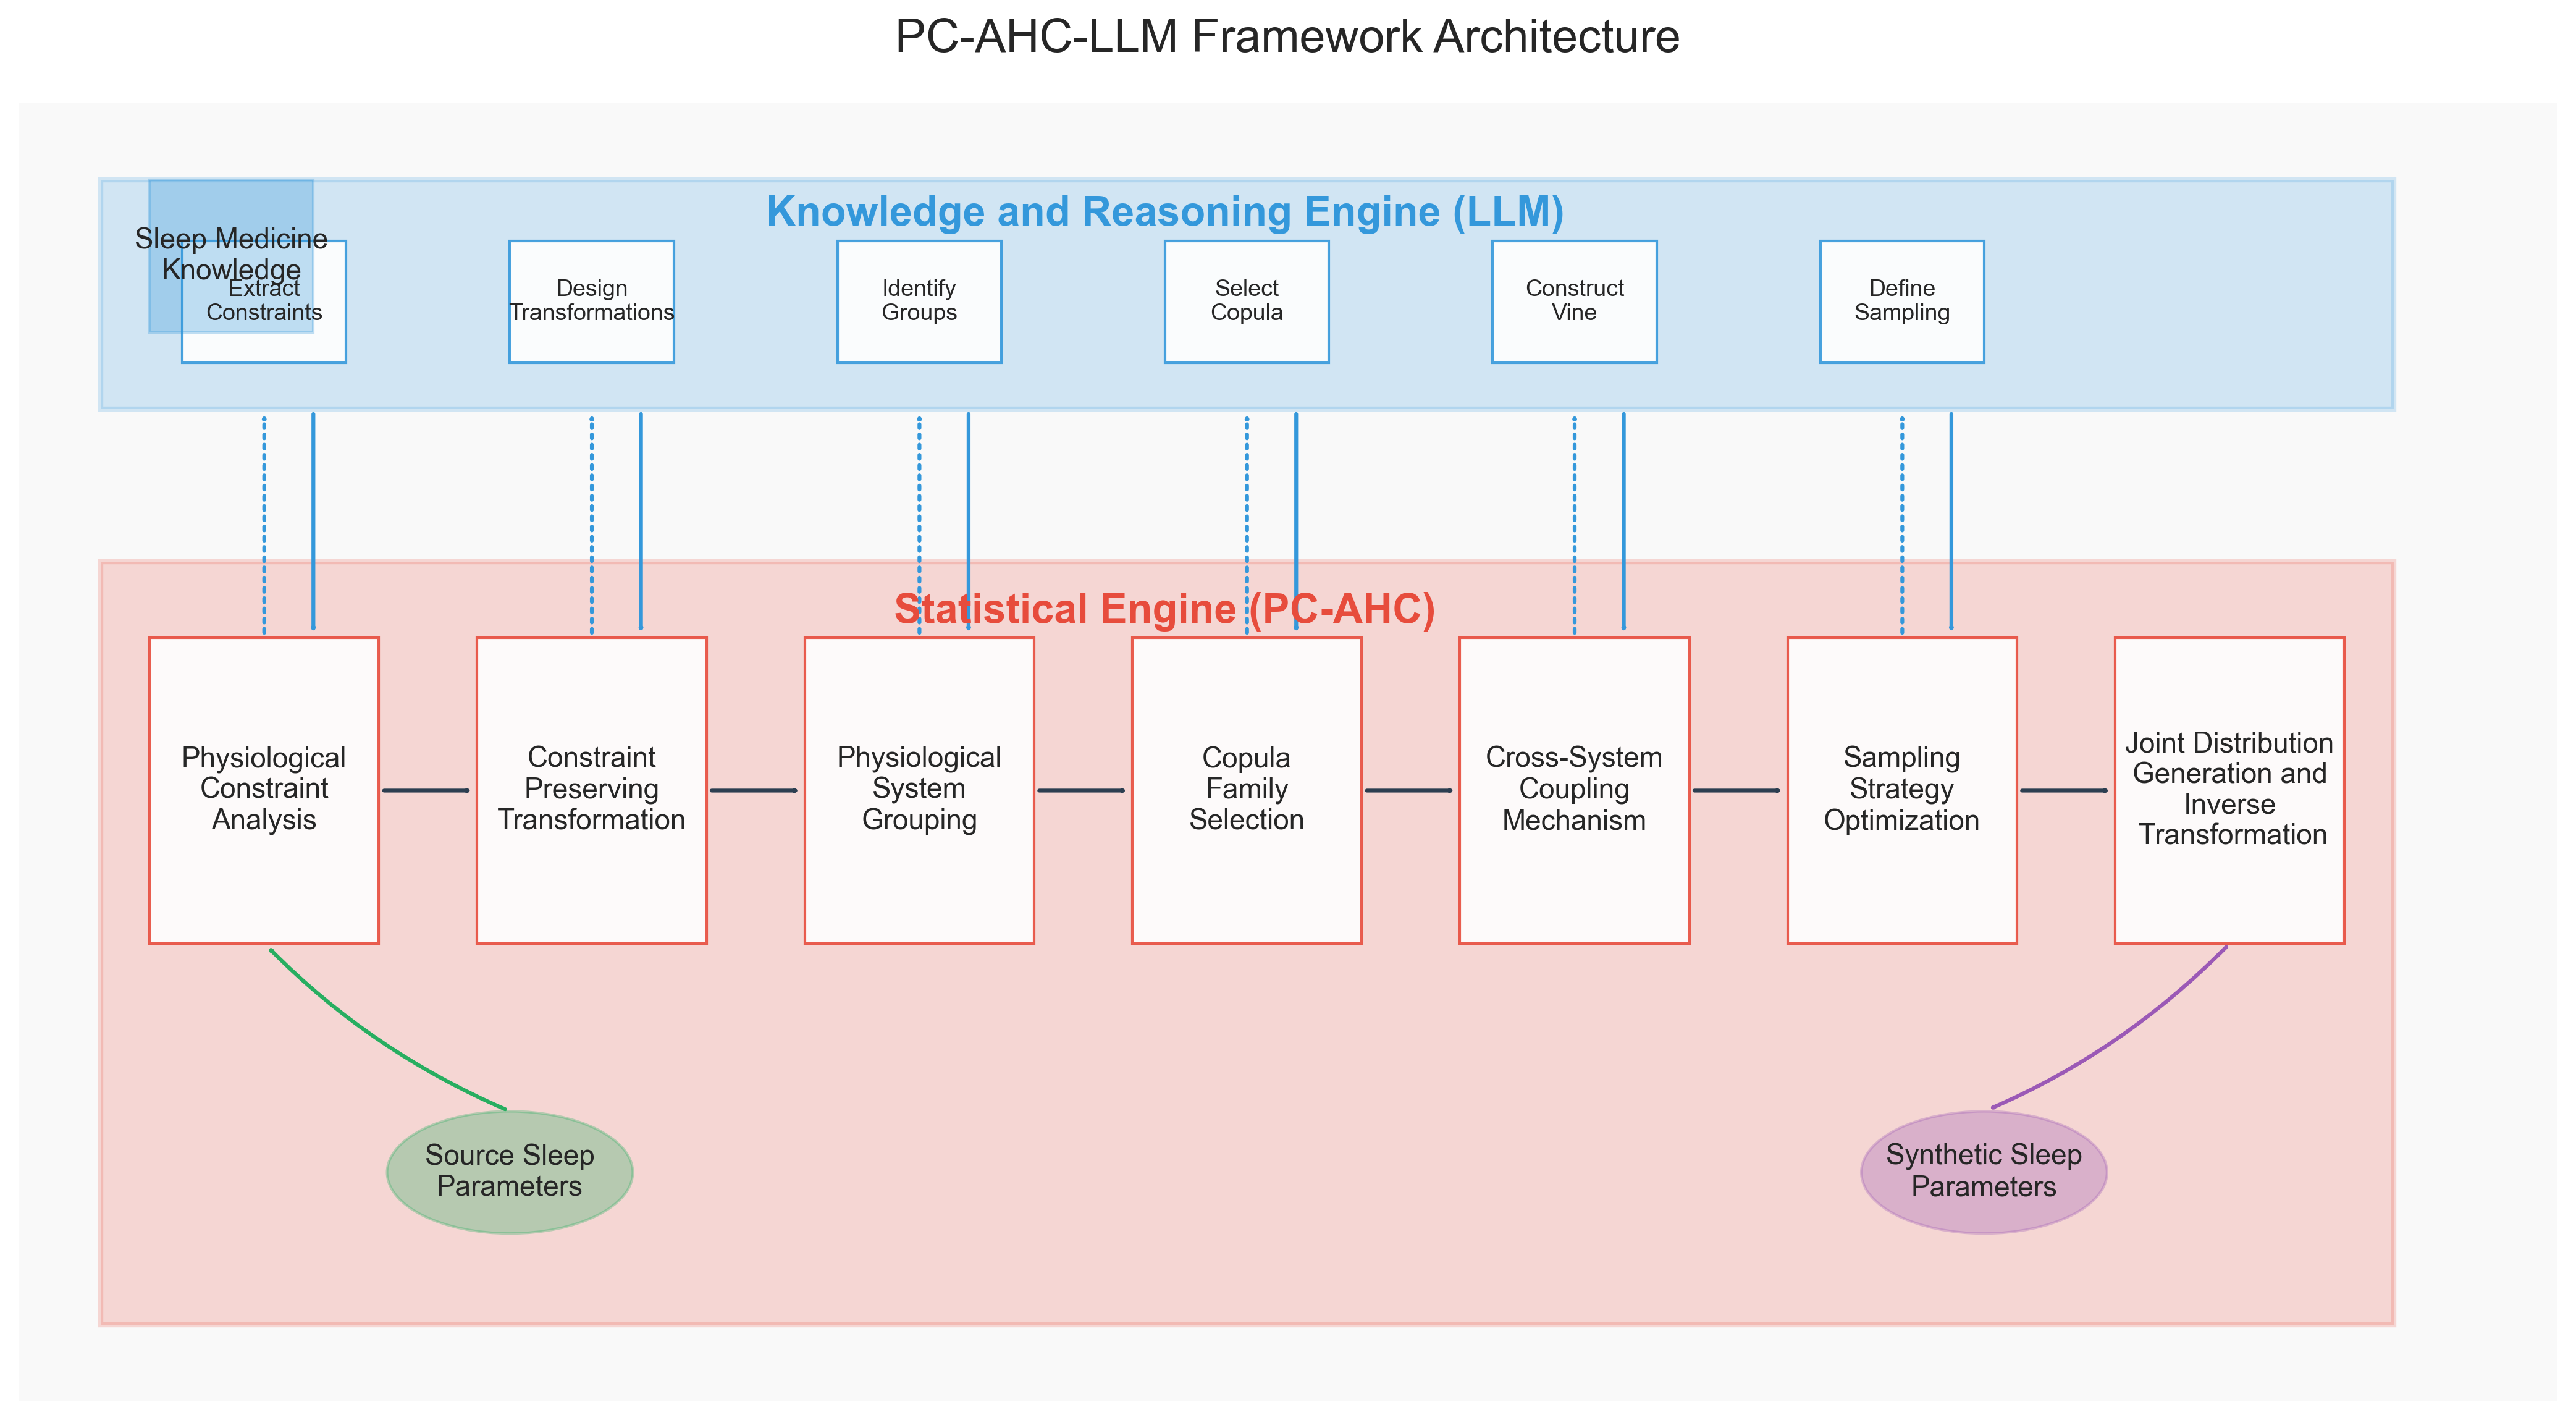
\includegraphics[width=\textwidth]{pc_ahc_llm_framework_final.png}
\caption{Overview of the PC-AHC-LLM framework. The Knowledge and Reasoning Engine (LLM) guides physiological constraint extraction, copula optimization, and sampling strategies, interacting synergistically with the Statistical Engine (PC-AHC) to generate physiologically-consistent synthetic sleep data.}
\label{PC-AHC-LLM}
\end{figure}
\begin{itemize}
\item \textbf{Statistical Engine (PC-AHC)}: Employs hierarchical copula models to capture complex statistical dependencies among physiological parameters.
\item \textbf{Knowledge and Reasoning Engine (LLM)}: Utilizes domain-specific physiological knowledge to guide constraint extraction, model optimization, and sampling strategies.
\end{itemize}

The workflow illustrated in Algorithm \ref{alg:pc-ahc-llm},integrates these components through three sequential stages: (1) physiological constraint extraction, (2) LLM-guided copula optimization, and (3) physiologically-guided sampling and synthesis.

\subsubsection{Physiological Constraint Extraction}

We leverage the LLM to systematically extract physiological constraints from authoritative sleep medicine literature. Formally, given a structured query template $\mathcal{Q}_{\text{constraints}}$, the LLM extracts a comprehensive set of constraints $\mathcal{C}$:
\begin{equation}
\mathcal{C} = \text{LLM}{\text{extractor}}( \mathcal{Q}{\text{constraints}})
\end{equation}

The extracted constraints include:

\begin{itemize}
\item \textbf{Sleep Architecture Constraints:}
\begin{align}
&\text{Deep Sleep Duration} + \text{Light Sleep Duration} \leq \text{Total Sleep Duration} \\
&\text{Total Sleep Duration} \in [3, 12],\text{hours},\quad \frac{\text{Deep Sleep Duration}}{\text{Total Sleep Duration}} \in [0.1, 0.35]
\end{align}

\item \textbf{Heart Rate Variability (HRV) Constraints:}
\begin{align}
    &\text{SDNN} \in [15, 220]\,\text{ms},\quad \text{RMSSD} \in [10, 180]\,\text{ms} \\
    &\text{PNN50} \in [0, 70]\%,\quad \text{LF/HF} \in [0.1, 7]
\end{align}

\item \textbf{Clinical Thresholds:}
\begin{align}
    &\text{SDNN} < 30\,\text{ms} \Rightarrow \text{Severe autonomic dysfunction} \\
    &\text{LF/HF} > 4 \Rightarrow \text{Sympathetic dominance}
\end{align}
\end{itemize}

Compared to traditional expert-defined rules, the LLM-driven extraction ensures greater comprehensiveness and physiological validity.

\subsubsection{LLM-Guided Copula Optimization}

Based on the extracted constraints, the LLM optimizes the copula modeling process through three key steps:

\paragraph{Optimal Variable Transformations} The LLM designs constraint-preserving transformations to standardize physiological parameters into latent Gaussian variables. In this study, sleep duration and HRV parameters are transformed via log-normalization and bounded scaling, ensuring physiological interpretability and statistical robustness.

\paragraph{Physiological Subsystem Grouping} The LLM identifies physiologically meaningful subsystems by analyzing inter-variable correlations and physiological pathways. Two subsystems are identified:

\begin{itemize}
    \item \textbf{Sleep Architecture Subsystem ($S_1$)}: Total sleep duration, deep sleep ratio, and light sleep ratio.
    \item \textbf{Autonomic Regulation Subsystem ($S_2$)}: SDNN, RMSSD, LF/HF, and PNN50.
\end{itemize}

\paragraph{Copula Family Selection.} For each subsystem, the LLM selects optimal copula families based on tail dependence metrics and physiological reasoning:

\begin{itemize}
\item \textbf{Subsystem ($S_1$)(Sleep Architecture)}: Gumbel copula (upper tail dependence), capturing synchronized increases in sleep components during recovery sleep.
\item \textbf{Subsystem ($S_2$) (Autonomic Regulation)}: Clayton copula (lower tail dependence), modeling concurrent dysregulation of HRV parameters during autonomic dysfunction.
\end{itemize}

Additionally, the LLM constructs a vine copula structure to model cross-subsystem dependencies, explicitly identifying critical conditional dependencies (e.g., RMSSD conditioned on deep sleep ratio) with physiologically-grounded justifications.

\subsubsection{Physiologically-Guided Sampling and Synthesis}

To ensure clinical relevance, the LLM defines a stratified sampling strategy emphasizing clinically significant parameter regions, such as short sleep duration (cardiovascular risk), low SDNN (autonomic dysfunction), high deep sleep ratio (optimal recovery), and elevated LF/HF ratio (sympathetic dominance). Importance weights are assigned based on clinical significance, guiding targeted sampling.

The synthetic data generation process involves:

\begin{enumerate}
\item Sampling correlated uniform variables from the optimized hierarchical copula structure.
\item Transforming these samples into standardized latent variables.
\item Applying inverse transformations to obtain physiologically valid synthetic parameters.
\end{enumerate}

This integrated approach combines the mathematical rigor of hierarchical copula modeling with the physiological expertise encoded by the LLM, resulting in synthetic sleep data that is both statistically robust and physiologically meaningful.

\begin{algorithm}[h]
\caption{PC-AHC-LLM Synthetic Sleep Data Generation}\label{alg:pc-ahc-llm}
\begin{algorithmic}[1]
\STATE \textbf{Input:} Source dataset $\mathcal{D}$, Domain knowledge $\mathcal{K}$
\STATE \textbf{Output:} Synthetic sleep parameter samples $\mathbf{X}_{\text{syn}}$

\STATE \textbf{Step 1: Extract Physiological Constraints using LLM}
\STATE \hspace{0.2cm} $\mathcal{C} \gets \text{LLM}_{\text{extractor}}(\mathcal{Q}_{\text{constraints}})$

\STATE \textbf{Step 2: Design Constraint-Preserving Transformations}
\STATE \hspace{0.2cm} $\mathcal{T} \gets \text{LLM}_{\text{designer}}(\mathcal{C}, \mathcal{D} \mid \mathcal{Q}_{\text{transformations}})$
\STATE \hspace{0.2cm} $\mathbf{Z} \gets \mathcal{T}(\mathcal{D})$

\STATE \textbf{Step 3: Identify Physiological Subsystems}
\STATE \hspace{0.2cm} $\mathcal{G} \gets \text{LLM}_{\text{clusterer}}(\mathbf{Z}, \mathcal{K} \mid \mathcal{Q}_{\text{grouping}})$
\STATE \hspace{0.2cm} Obtain subsystems: $S_1, S_2, \dots, S_m$

\STATE \textbf{Step 4: Select Optimal Copula Families for Each Subsystem}
\FOR{each subsystem $S_i \in \mathcal{G}$}
    \STATE Compute dependence metrics $(\lambda_U^{(i)}, \lambda_L^{(i)}, \gamma^{(i)})$
    \STATE Select copula family: $\mathcal{C}_{S_i} \gets \text{LLM}_{\text{classifier}}(\lambda_U^{(i)}, \lambda_L^{(i)}, \gamma^{(i)}, \mathcal{K})$
\ENDFOR

\STATE \textbf{Step 5: Construct Cross-Subsystem Vine Structure}
\STATE \hspace{0.2cm} $\mathcal{V} \gets \text{LLM}_{\text{structure}}(\mathbf{Z}, \mathcal{K} \mid \mathcal{Q}_{\text{vine}})$

\STATE \textbf{Step 6: Define Physiologically-Guided Sampling Strategy}
\STATE \hspace{0.2cm} $\mathcal{S} \gets \text{LLM}_{\text{sampler}}(\mathcal{D}, \mathcal{K} \mid \mathcal{Q}_{\text{sampling}})$

\STATE \textbf{Step 7: Generate Synthetic Samples}
\STATE \hspace{0.2cm} Sample correlated uniform variables: $\mathbf{U} \sim \mathcal{V}(\mathcal{C}_{S_1}, \dots, \mathcal{C}_{S_m})$
\STATE \hspace{0.2cm} Transform to latent Gaussian variables: $\mathbf{Z}_{\text{syn}} \gets \Phi^{-1}(\mathbf{U})$
\STATE \hspace{0.2cm} Apply inverse transformations: $\mathbf{X}_{\text{syn}} \gets \mathcal{T}^{-1}(\mathbf{Z}_{\text{syn}})$

\STATE \textbf{return} Synthetic sleep parameter samples $\mathbf{X}_{\text{syn}}$
\end{algorithmic}
\end{algorithm}


\subsection{Data Preparation}
\subsubsection{Data Collection}
Wearable devices capture electrocardiogram (ECG) signals during sleep. These signals are used to derive heart rate variability (HRV) parameters, providing insights into autonomic nervous system activity and sleep quality. HRV metrics are essential for personalized sleep health analysis and recommendation generation. We collected real ECG data from a population-based sleep study to establish a robust dataset. We recruited 160 participants from Jinan University and collected sleep ECG data using the Bodyguard 2 device (Firstbeat Technologies Ltd., Finland), a lightweight, wearable ECG monitor (24 g, 47 mm × 63 mm × 10.6 mm) with a rechargeable Li-Poly battery, offering continuous long-term recording and 128 MB storage capacity. We recorded ECG signals at a sampling rate of 1000 Hz, ensuring high precision for HRV analysis. The study was approved by the Ethics Committee of the First Affiliated Hospital of Jinan University (Approval Number: KY-2023299) and conducted in accordance with the Declaration of Helsinki.
HRV features were extracted following standard methods, resulting in a dataset for analyzing sleep-related cardiac dynamics. In this study, we focus on four key metrics—SDNN (Standard Deviation of NN intervals), RMSSD (Root Mean Square of Successive Differences), LF/HF (Low Frequency/High Frequency ratio), and PNN50 (Percentage of NN intervals greater than 50 ms)—which are crucial for assessing autonomic nervous system regulation during sleep. Following a review by a professional physician, data anomalies, including improper wear, device detachment, and abnormal readings, were excluded. After data cleaning, the final dataset consisted of 115 valid recordings. 

\subsubsection{Data synthesis}
To overcome limitations in data volume and diversity, we utilized data synthesis techniques, generating additional data based on predefined distribution rules and insights from large models. The framework shown in Fig. \ref{fig3} outlines the process of generating synthetic datasets, starting from the collection and processing of anchor data, followed by the application of physiological parameter constraints. This approach ensures that the synthesized data closely mimics real-world conditions. The framework also includes steps for generating personalized recommendations and potential user questions based on the synthesized sleep reports, thereby creating a comprehensive and realistic dataset for model training and evaluation.
\begin{figure}[ht]
\centering
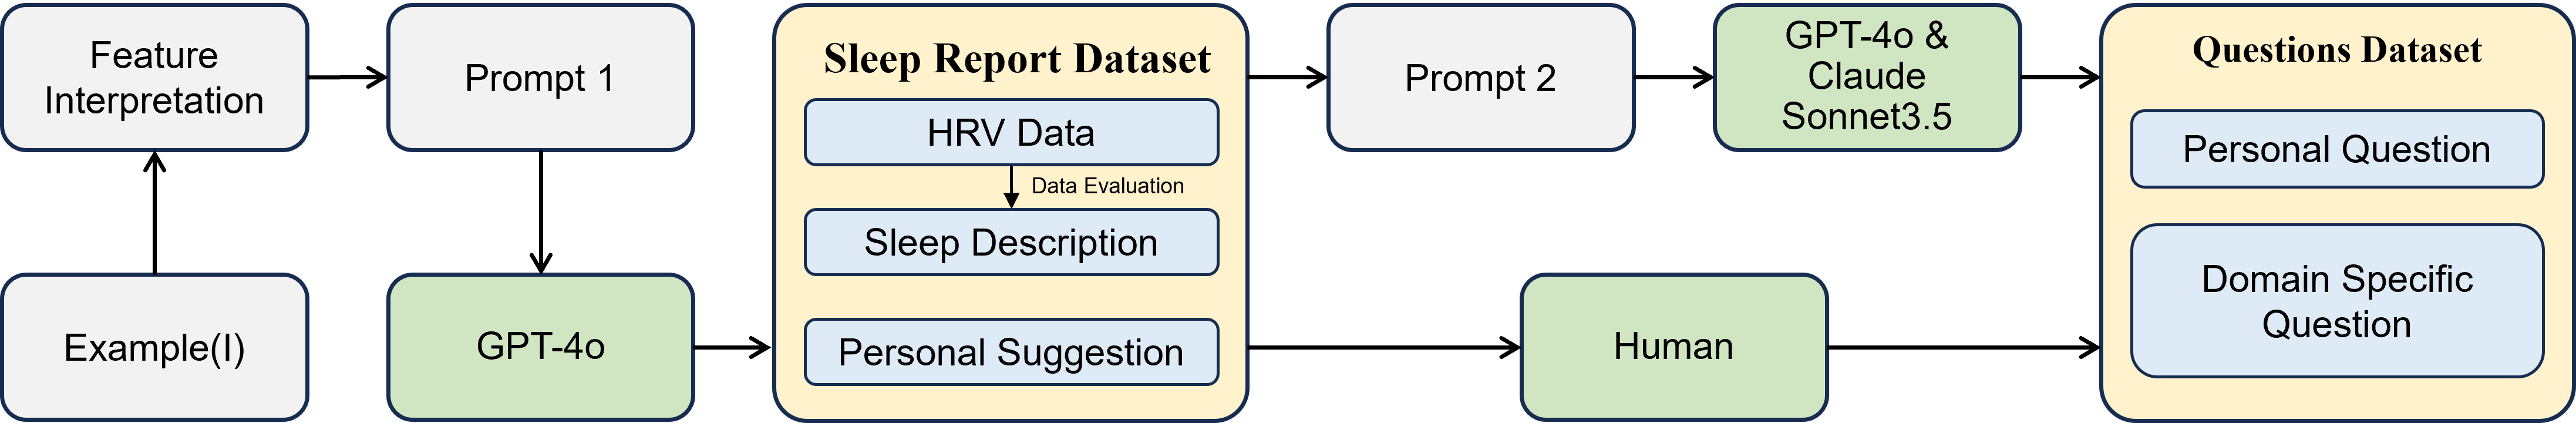
\includegraphics[width=\columnwidth]{datasyhths1.png}
\caption{The comprehensive process of data synthesis, including the generation of wearable data (HRV), sleep descriptions, and personalized suggestions using GPT-4o. These elements form a complete sleep report, which is then used to create personalized questions and sleep-related knowledge inquiries through both human and LLM (GPT-4o and Claude Sonnet 3.5) interactions.}
\label{fig3}
\end{figure}

Using GPT-4o, we synthesized 1000 samples derived from real-world examples and predefined physiological rules. Each sample includes HRV parameters recorded throughout the sleep period, including key metrics such as SDNN and RMSSD, alongside sleep duration and sleep staging data. To assess users' cardiac health, stress resilience, and other related conditions, we employed predefined algorithms analogous to those described in prior studies. These algorithms facilitated the generation of comprehensive sleep state assessments, which were subsequently integrated with the corresponding sample data. Leveraging GPT-4o, personalized recommendations were then generated based on these combined assessments, providing tailored guidance specific to the evaluated sleep profiles.

The Algorithm \ref{data_synthesis} illustrates the detailed process of synthesizing data. $\mathbf{D_A}$ represents the predefined evaluation algorithm, \(Pr\) represents the predefined prompt template, while Table \ref{tab:template1} and Table \ref{tab:template2} provide example prompts for \(Pr1\) and \(Pr2\).  \(I\) represents the HRV data derived from real data collected during the user’s monitoring. \(R\), which is shown in Algorithm \ref{synthesis_rule}, represents the rule guiding GPT-4o in synthesizing wearable data, following a structured approach.
\begin{algorithm}[h]
\caption{Data Synthesis for Sleep Analysis}\label{data_synthesis}
\begin{algorithmic}
\STATE \hspace{0.0cm} \textbf{Input:} Sample $\mathbf{I}$, Rule $\mathbf{R}$
\STATE \hspace{0.0cm} \textbf{Output:} Personalized suggestion $\mathbf{S}$, Personalized questions $\mathbf{Q}$
\STATE \hspace{0.0cm} \textbf{Step 1: Generate wearable data using GPT-4o}
\STATE \hspace{0.1cm} $\mathbf{wearable\_data} \gets \mathrm{GPT\text{-}4o}(\mathrm{Pr1}(\mathbf{I} + \mathbf{R}))$
\STATE \hspace{0.0cm} \textbf{Step 2: Describe sleep based on wearable data}
\STATE \hspace{0.1cm} $\mathbf{sleep\_description} \gets \mathbf{D_A}(\mathbf{wearable\_data})$
\STATE \hspace{0.0cm} \textbf{Step 3: Generate personal suggestion using GPT-4o}
\STATE \hspace{0.1cm} $\mathbf{S} \gets \mathrm{GPT\text{-}4o}(\mathrm{Pr2}(\mathbf{wearable\_data} + \mathbf{sleep\_description}))$
\STATE \hspace{0.0cm} \textbf{Step 4: Generate personalized questions using GPT-4o and Claude Sonnet 3.5}
\STATE \hspace{0.1cm} $\mathbf{Q} \gets \mathrm{GPT\text{-}4o}(\mathbf{S}) + \mathrm{Claude\text{-}Sonnet\text{-}3.5}(\mathbf{S})$
\STATE \hspace{0.1cm} \textbf{return} Personalized suggestion $\mathbf{S}$, Personalized questions $\mathbf{Q}$
\end{algorithmic}
\end{algorithm}

\begin{table}[ht]
\centering
\caption{Wearable Data Production}
\label{tab:template1}
\begin{tabular}{@{}p{1\textwidth}@{}}
\toprule
\textbf{Instruction Template1:} \\[2mm]
The anchor \{I\} represents the HRV data derived from real data collected during the user's monitoring. Please generate data following the rules outlined in Algorithm~\ref{synthesis_rule}, ensuring that it captures various sleep health conditions across the population. Ensure that the parameters in the reports reflect realistic and plausible health states without impossible or contradictory conditions. Additionally, pay attention to the diversity and faithfulness of the report content, avoiding repetition. Each report should start with "HRV DATA:".
\\[1mm]
\bottomrule
\end{tabular}
\end{table}

\begin{table}[ht]
\centering
\caption{Personalized Suggestion Production}
\label{tab:template2}
\begin{tabular}{@{}p{1\textwidth}@{}}
\toprule
\textbf{Instruction Template2:} \\[2mm]
You are a sleep expert. Please generate personalized recommendations based on the following HRV data and sleep description. The recommendation should address: (1) Sleep Overview; (2) Cardiac Health; (3) Stress and Stress Resilience; (4) Sleep Apnea and Sleep Interruptions. Include relevant parameters (SDNN, RMSSD, LF/HF, PNN50) and their descriptions.
\\[1mm]
\bottomrule
\end{tabular}
\end{table}


After generating the personalized recommendations, GPT-4o was utilized to create a set of likely questions based on the sleep reports, which included both physiological parameters and personalized advice. For each of the 100 sleep reports, 15 personalized questions were generated, resulting in a total of 16,725 personalized questions. It is important to note that when generating questions using GPT-4o, the 100 user reports were sequentially input in the form of multi-turn dialogues.This method reduces the likelihood of generating repetitive questions while promoting greater diversity in the generated queries. By doing so, it ensures a broader and more varied set of questions, effectively reflecting the complexities of real-world interactions. In addition, GPT-4o was also employed to generate 2,000 sleep-related knowledge questions. Furthermore, Claude-Sonnet 3.5 was used to produce an additional 100 domain-specific knowledge questions. The prompt to produce wearable data, personalized suggestions and questions are shown in Table \ref{template3}.
\begin{table}[t]
\centering
\caption{Personalized Question Production}
\label{template3}
\begin{tabular}{@{}p{1\textwidth}@{}}
\toprule
\textbf{Instruction Template3:} \\[2mm]
"You are a sleep medicine expert. Generate 150 questions that users are most likely to ask based on each sleep quality report. The questions should mainly revolve around personalized details (e.g., 'Is my SDNN value normal?') and should not include specific numerical values. Ensure diversity in phrasing, and all outputs should start with 'Question 1:' containing only the question content."
\\[1mm]
\bottomrule
\end{tabular}
\end{table}

\subsection{Profile-Guided Distillation of Expert Reasoning}

In this section, we introduce the \textbf{Profile-Guided Distillation of Expert Reasoning (ProDREAM)} framework, as illustrated in Fig.~\ref{LoRA-MoE}. ProDREAM leverages \textbf{profile-guided lightweight Chain-of-Thought (CoT) prompting} and \textbf{LoRA-based Mixture of Experts (MoE) distillation} to enhance the performance of a compact language model across three core tasks: \textit{sleep report generation}, \textit{personalized question-answering}, and \textit{domain-specific knowledge answering} (see Algorithm~\ref{ESCaLE_distillation}). These tasks are instruction-based fine-tuned simultaneously, ensuring task-specific optimization.

\subsubsection{Profile-Guided Lightweight Chain-of-Thought (PG-LCoT)}

The proposed \textbf{Profile-Guided Lightweight Chain-of-Thought (PG-LCoT)} extends traditional CoT reasoning by incorporating user-specific sleep profiles into structured reasoning templates. This approach enables personalized and adaptive reasoning tailored to individual sleep characteristics. Formally, PG-LCoT is defined as:

\[
\mathcal{T}(p) = \sum_{i=1}^{3} \alpha_i(p) \cdot \text{CoT}_i(p) + \text{Profile}(p)
\]

Here, $\mathcal{T}(p)$ represents the personalized reasoning chain for a user with profile $p$, $\text{CoT}_i(p)$ denotes task-specific reasoning templates modified by profile characteristics, $\alpha_i(p)$ are profile-dependent weighting coefficients, and $\text{Profile}(p)$ encodes key sleep pattern information. The user profile vector captures critical sleep parameters, expressed as:

\[
\text{Profile}(p) = [s_{\text{duration}}, s_{\text{efficiency}}, s_{\text{latency}}, s_{\text{fragmentation}}, s_{\text{REM}}, s_{\text{deep}}, s_{\text{consistency}}]
\]
For certain users, if any parameter is unavailable due to missing data or incomplete records, the corresponding entry in the profile vector is set to \textit{null}. This ensures that the model can handle incomplete profiles gracefully while maintaining robustness in downstream tasks.

This profile-guided reasoning introduces two key innovations:
\begin{enumerate}
    \item \textbf{Profile-Specific Reasoning Paths}:  
    The reasoning structure dynamically adapts to detected sleep disorders or patterns. For instance, users with insomnia profiles are guided through templates emphasizing psychological and behavioral factors, while users with apnea profiles are directed toward templates focusing on physiological metrics such as oxygen saturation and respiratory patterns.

    \item \textbf{CoT Composition}:  
    Instead of relying on fixed templates, we distill reasoning patterns from a teacher model into a compositional template library $\mathcal{L}$, organized by task type and profile characteristics:
    \begin{equation}
    \mathcal{L} = \{\text{CoT}_{i,j} \mid i \in \text{Tasks}, j \in \text{ProfileClusters}\}
    \end{equation}
    A profile-guided attention network computes relevance scores between the input query, user profile, and template library:
    \[
    \text{Score}(q, p, \text{CoT}_{i,j}) = \text{MLP}([\text{Enc}(q); \text{Enc}(p); \text{Enc}(\text{CoT}_{i,j})])
    \]
    These scores determine the selection and emphasis of reasoning components during inference, ensuring coherence while incorporating personalized considerations derived from sleep profiles.
\end{enumerate}

\subsubsection{Task-Specific Adaptations}

For each of the three tasks, we tailored the CoT structure to align with task-specific requirements. The tasks are defined as follows:

\begin{itemize}
    \item \textbf{Sleep Report Generation}:  
    This task involves generating a standardized sleep report based on physiological signals collected during sleep. The report is structured according to predefined content categories, including sleep stages, sleep efficiency, and other key metrics. The process concludes with personalized recommendations tailored to the user's specific sleep patterns and needs.

    \item \textbf{Personalized Question-Answering}:  
    This task addresses user-specific queries related to their sleep state and the generated sleep report. The questions are typically grounded in the user's personal sleep data, and the answers are designed to provide actionable insights or clarifications based on their unique sleep profile.

    \item \textbf{Domain-Specific Knowledge Answering}:  
    This task focuses on answering general questions about sleep-related knowledge that are independent of the user's personal state or sleep data. The goal is to provide accurate and comprehensive responses to queries about sleep science, health, and best practices.
\end{itemize}

To address the unique requirements of these tasks, we designed task-specific CoT structures:

\begin{itemize}
    \item \textbf{Sleep Report Generation}:  
    The CoT reasoning begins with analyzing raw physiological signals, correlates patterns with sleep stages, contextualizes findings with personal profile, and concludes with personalized recommendations. This structured reasoning ensures that the generated report is both comprehensive and tailored to the user's needs.

    \item \textbf{Personalized Question-Answering}:  
    The CoT grounds responses in the user's profile, incorporates contextual history from the sleep report, and emphasizes profile-specific factors to deliver tailored answers. This approach ensures that the answers are relevant and actionable for the user.

    \item \textbf{Domain-Specific Knowledge Answering}:  
    The CoT starts with general knowledge retrieval from the model's knowledge base, followed by profile-guided contextualization to adapt educational content to the user's specific sleep challenges. This ensures that the responses are both accurate and aligned with the user's understanding level.
\end{itemize}

\subsubsection{Efficient Distillation via LoRA-Based MoE}

To optimize the PG-LCoT approach for a compact 0.5B parameter model, we distilled reasoning patterns from a teacher model (Qwen-max) using LoRA-based Mixture of Experts (MoE) techniques. By analyzing the teacher model's reasoning paths across diverse sleep analysis scenarios, we formalized lightweight templates that preserve essential reasoning structures while reducing token length by 30-50\%. This compression ensures that the distilled model maintains high performance while being computationally efficient.

\subsubsection{Integration with MoE Architecture}

The proposed PG-LCoT approach seamlessly integrates with our LoRA-based MoE architecture. The user profile information not only guides CoT template selection but also influences the router's expert assignment:

\begin{equation}
\mathbf{g}(\mathbf{h}_t, \mathbf{p}) = \mathbf{W}{\text{gate}}\mathbf{h}t + \mathbf{W}{\text{profile}}\mathbf{p} + \mathbf{b}_{\text{gate}}
\label{eq:gate_profile}
\end{equation}

Where $\mathbf{p}$ represents the user profile embedding and $\mathbf{W}{\text{profile}}$ is a learned matrix mapping profile information to routing decisions. This ensures that both the reasoning process and expert activation are coherently aligned with user characteristics.

In our experiments, we configured six LoRA-based expert adapters, each specialized for distinct functions: knowledge, data analysis and feature extraction, report generation, report understanding and correlation, personalized Q\&A, and sleep knowledge Q\&A. The router was set to $k=3$, activating three expert adapters per input. Specifically:
\begin{itemize}
\item The knowledge adapter was always active as a foundational component.
\item Report generation activated the data analysis and report generation adapters.
\item Personalized Q\&A engaged the report understanding and personalized Q\&A adapters.
\item Sleep knowledge Q\&A utilized the sleep knowledge and report understanding adapters.
\end{itemize}

\subsubsection{Expert Configuration}

The MoE architecture contains six specialized LoRA adapters ($
r=16$ rank) with dimensional relationships:

\begin{equation}
\mathbf{W}{\text{gate}} \in \mathbb{R}^{d{\text{in}} \times N}, \quad d_{\text{in}}=768, \quad d_{\text{expert}}=256
\end{equation}

\begin{table}[h]
\centering
\caption{Expert Adapter Specialization}
\begin{tabular}{ll}
\hline
Adapter & Function Domain \\ \hline
$\mathcal{E}_1$ & Data Analysis \& Feature Extraction \\
$\mathcal{E}_2$ & Report Generation \\
$\mathcal{E}_3$ & Report Understanding \& Correlation \\
$\mathcal{E}_4$ & Personalized Q\&A \\
$\mathcal{E}_5$ & Sleep domain Q\&A \\
$\mathcal{E}_6$ & knowledge \\ \hline
\end{tabular}
\end{table}

\subsubsection{Dynamic Weight Allocation}
The router dynamically assigns weights ($W$) to each adapter. The routing mechanism employs a temperature-controlled softmax function with top-k selection:

\begin{equation}
    p_i = \frac{\exp(g_i/\tau)}{\sum_{j=1}^N \exp(g_j/\tau)} \quad 
    \text{(temperature-scaled probability, } \tau > 0\text{)}
    \label{eq:prob}
\end{equation}

\begin{equation}
    \mathbf{W} = \mathbf{p} \circ \mathbf{M}_{\text{sparse}} \quad
    \text{(sparse weight selection)}
    \label{eq:sparse_weight}
\end{equation}

\begin{equation}
    \mathbf{M}_{\text{sparse}} = \mathop{\text{OneHot}}\big(\mathop{\text{argtopk}}(\mathbf{p}, k=3)\big) \in \{0,1\}^N
    \label{eq:mask_def}
\end{equation}

\noindent where $h_t \in \mathbb{R}^{d_{in}}$ is the hidden state at position $t$, $N = 6$ experts, and $k = 3$ activated experts per token. As an example, as illustrated in Figure \ref{LoRA-MoE}, for the personalized question "How can I improve my stress resilience through psychological regulation?", after loading the profile-guided CoT and tokenization, the router activates the Data Analysis \& Feature Extraction, Personalized QA, and Knowledge adapters, assigning weights of 0.3, 0.5, and 0.2, respectively.

Outputs from the adapters were processed through a Cross-Attention Layer and integrated with the transformer layers of the base model, Qwen2.5 0.5B.

\subsubsection{Loss Formulation}
To mitigate load imbalance among expert adapters due to varying task sample sizes and the top-k routing mechanism, we incorporated an auxiliary loss alongside the standard cross-entropy loss as a regularization term. We also introduced a profile alignment loss to ensure consistency between CoT reasoning and user profiles:

\begin{equation}
L_{\text{profile}} = \lambda_p \sum_{i} \text{KL}(P_{\text{CoT}i}(p) \parallel P{\text{adapter}_i}(p))
\end{equation}

Where $P_{\text{CoT}}(p)$ represents the probability distribution over reasoning paths given profile $p$, and $P_{\text{adapter}}(p)$ is the adapter activation distribution. This loss ensures coherence between reasoning and model specialization.

The \textbf{auxiliary load balancing loss} encourages an even distribution of task load across experts:
\begin{equation}
L_{\text{aux}} = \lambda_a \sum_{i} \left( \left| F_i - \frac{1}{N} \right|^2 + \left| P_i - \frac{1}{N} \right|^2 \right)
\end{equation}

where $F_i$ represents the fraction of tokens assigned to expert $i$. $P_i$ represents the fraction of router probability allocated to expert $i$. $N$ is the total number of experts. $\lambda_a$ is a regularization parameter controlling the strength of load balancing.

The \textbf{activation frequency regularization loss} ensures uniform activation of all experts:
\begin{equation}
L_{\text{freq}} = \lambda_f \sum_{i} \left( \text{activation}_i - \frac{T}{N} \right)^2
\end{equation}
where $\text{activation}_i$ is the number of times expert $i$ is activated. $T$ is the total number of activations. $N$ is the total number of experts.

The total loss function is a weighted sum of the components:
\begin{equation}
L_{\text{total}} = L_{\text{CE}} + \alpha \cdot L_{\text{aux}} + \beta \cdot L_{\text{freq}} + \gamma \cdot L_{\text{profile}}
\end{equation}

Where $L_{CE}$ is the \textbf{cross-entropy loss} for prediction accuracy. In this experiment, the coefficients $\alpha$, $\beta$, and $\gamma$ were set to 0.1, 0.15, and 0.05, respectively, to balance the contributions of each loss component.

\subsubsection{Routing Algorithm}
The profile-guided route process follows Algorithm \ref{alg:router}:
\begin{algorithm}
\caption{Profile-Guided Router Implementation}
\label{alg:router}
\begin{algorithmic}[1]
\REQUIRE Hidden states $\mathbf{H} \in \mathbb{R}^{B \times S \times d_{\text{in}}}$, User profiles $\mathbf{P} \in \mathbb{R}^{B \times d_{\text{profile}}}$
\REQUIRE Parameters: $\tau=0.1,\ k=3,\ N=6$
\STATE Encode user profiles: 
   $\mathbf{P}_{\text{enc}} = \text{ProfileEncoder}(\mathbf{P}) \in \mathbb{R}^{B \times d_{\text{profile\_enc}}}$
\STATE Compute profile-aware gate logits: 
   $\mathbf{G} = \mathbf{H}\mathbf{W}_{\text{gate}} + \mathbf{P}_{\text{enc}}\mathbf{W}_{\text{profile}} + \mathbf{b}_{\text{gate}}$
\STATE Apply temperature scaling: 
   $\mathbf{G} \leftarrow \mathbf{G}/\tau$
\STATE Compute expert probabilities: 
   $\mathbf{P}_{\text{exp}} = \text{softmax}(\mathbf{G})$
\STATE Select top-$k$ experts: 
   $\mathbf{W}, \mathbf{I} = \underset{k\text{-max}}{\text{argtop}}(\mathbf{P}_{\text{exp}})$
\STATE Normalize weights: 
   $\mathbf{W} \leftarrow \mathbf{W}/\|\mathbf{W}\|_1$
\STATE Compute total loss: $\mathcal{L}_{\text{total}}$ including profile alignment
\ENSURE Activated weights $\mathbf{W}$, indices $\mathbf{I}$, loss $\mathcal{L}_{\text{total}}$
\end{algorithmic}
\end{algorithm}

\begin{figure}[t]
\centering
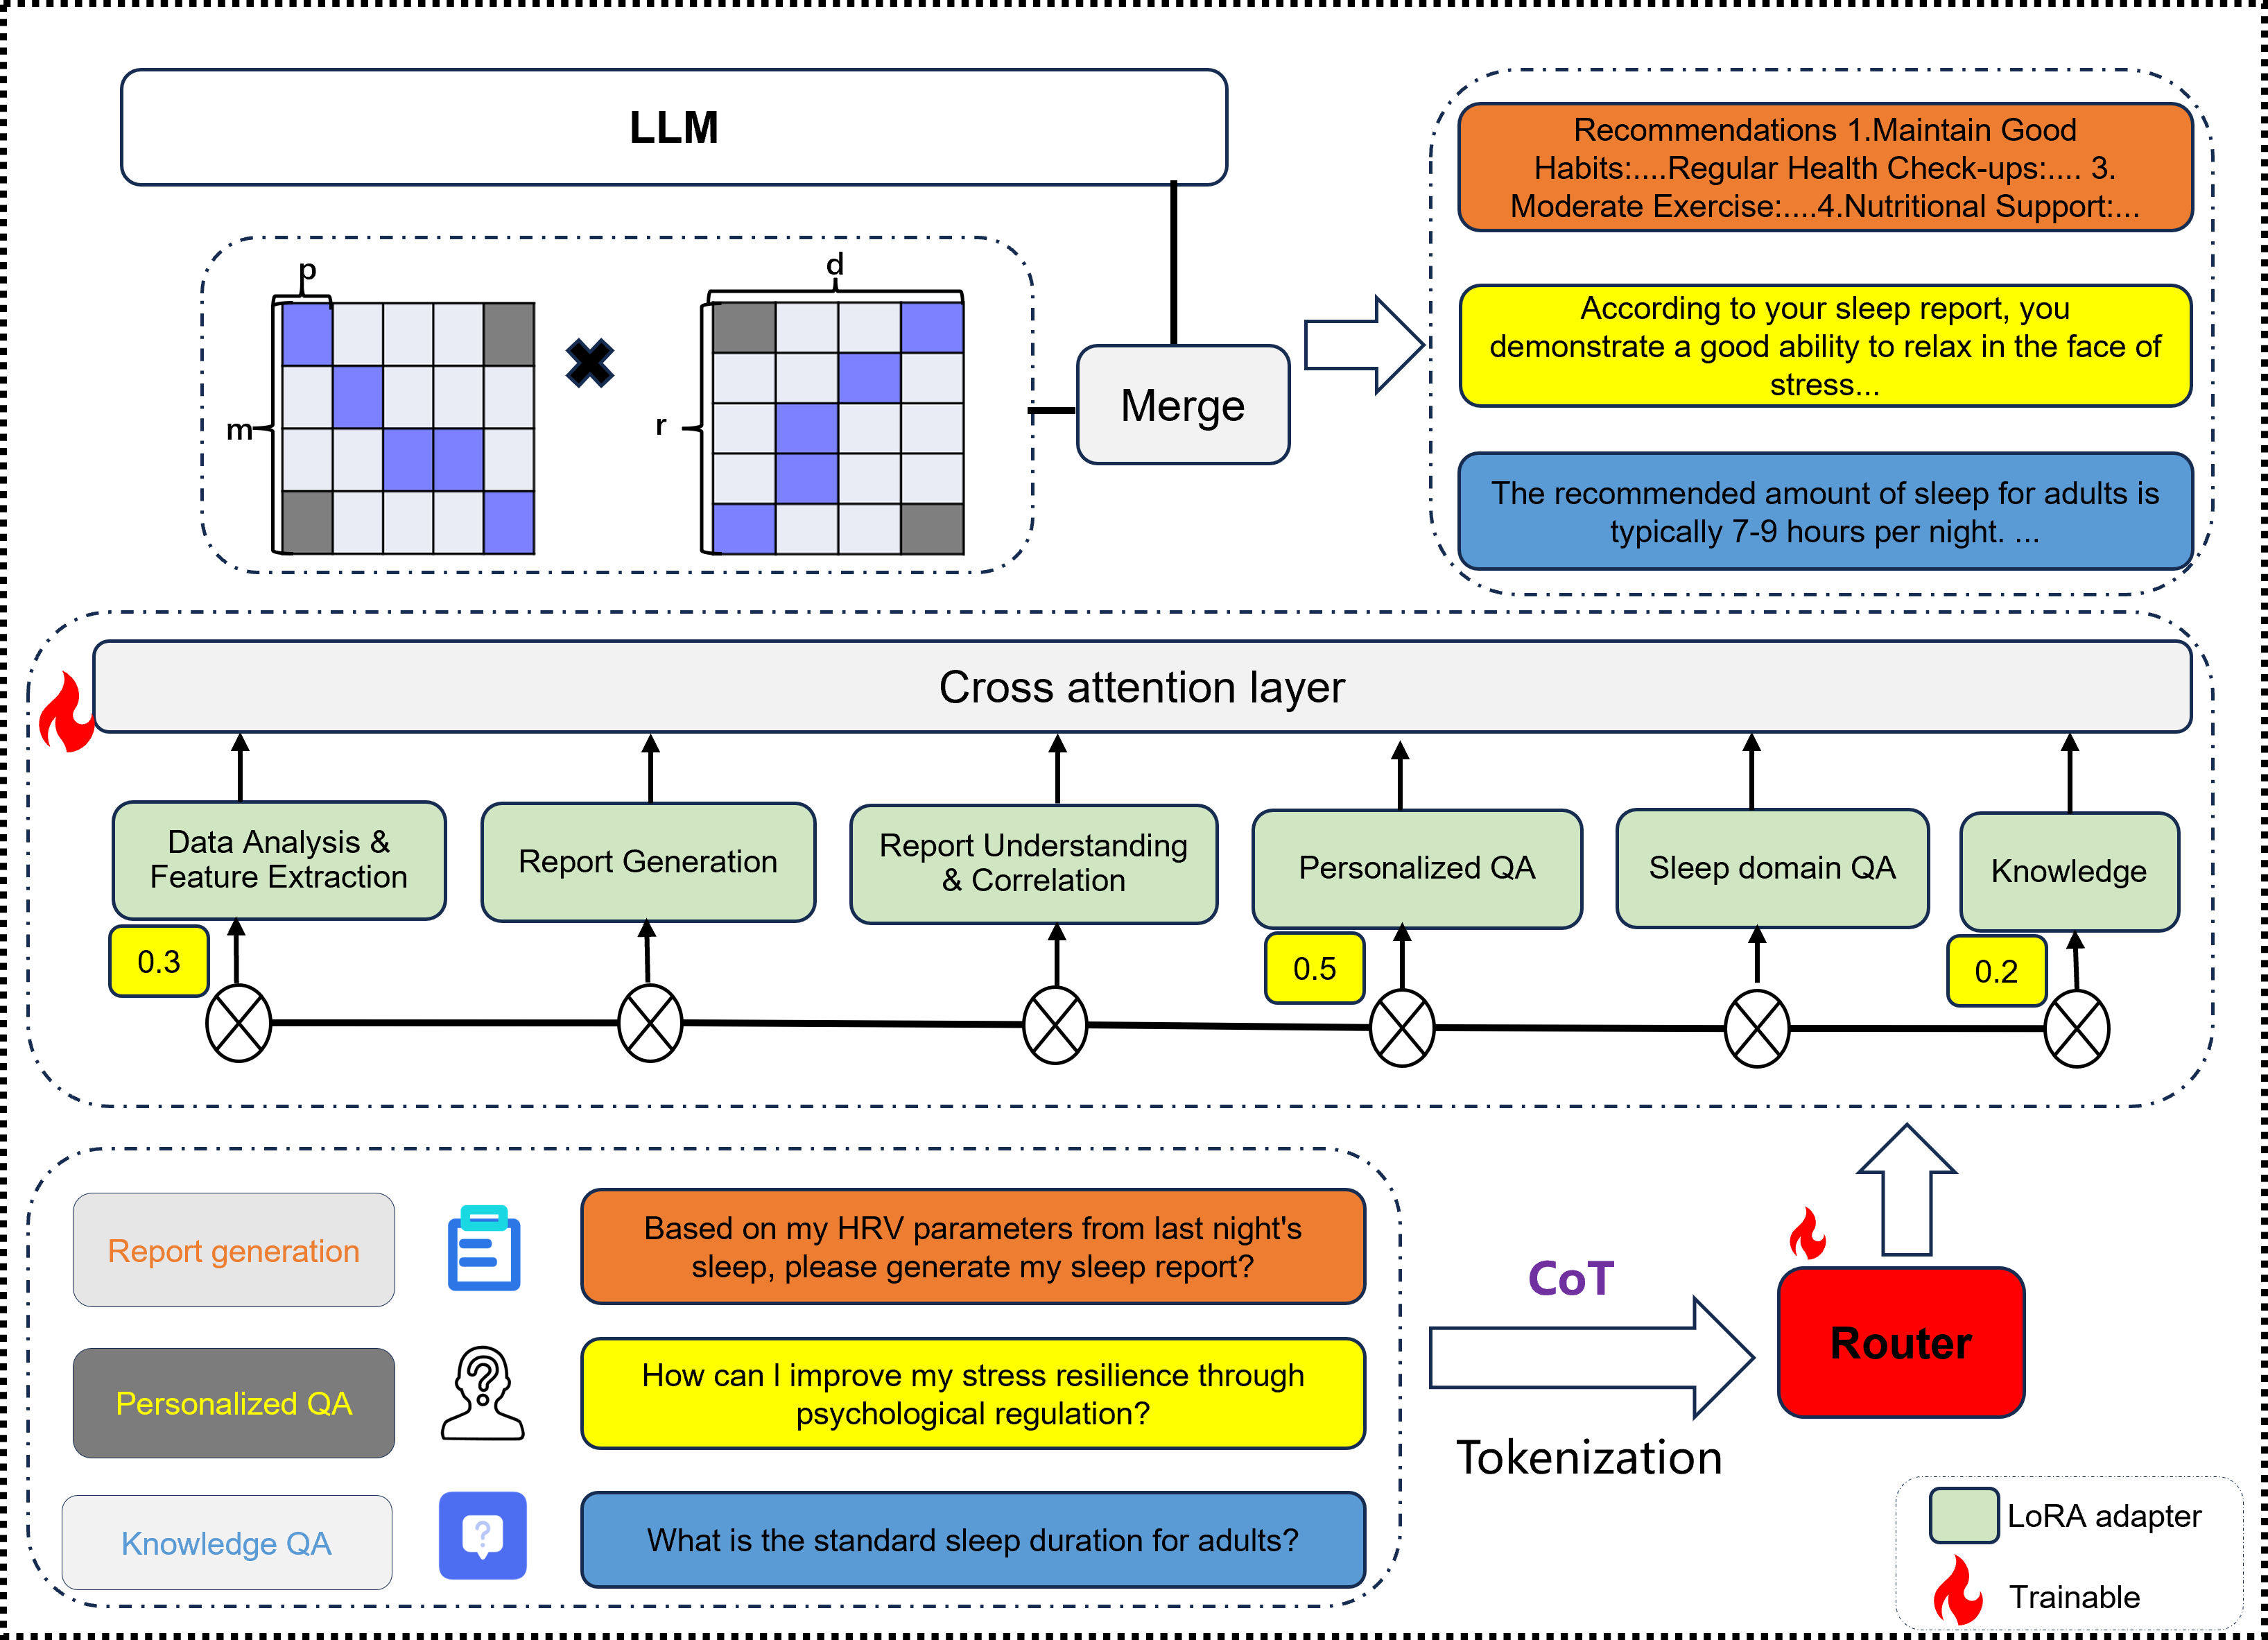
\includegraphics[width=\textwidth]{MoELORA5.png}
\caption{The architecture of ESCaLE, where the input is routed through a dynamic activation mechanism that assigns weights to different adapters. Notably, the knowledge adapter is activated during every inference to provide shared knowledge across three tasks. The activated adapters are then fused via cross-attention mechanisms, and the resulting representations are integrated with the corresponding matrices in the transformer layer of base model.}
\label{LoRA-MoE}
\end{figure}

\begin{algorithm}[h]
\caption{CoT Distillation with LoRA-Based Mixture of Experts for ESCaLE Model}
\label{ESCaLE_distillation}
\begin{algorithmic}[1]
\STATE \textbf{TRAIN}$(\mathbf{X}, \mathbf{T})$
\STATE \textbf{Input:} Multi-task data $\mathbf{X}$ and teacher model Qwen-max $\mathbf{T}$
\STATE \textbf{Output:} Distilled student model ESCaLE
\STATE Initialize adapter and router parameters $\mathbf{\theta}$
\FOR{each batch $\mathbf{x}$ in $\mathbf{X}$}
  \STATE Generate teacher response: $\hat{\mathbf{y}} \gets \mathbf{T}(\mathbf{x})$
  \STATE $(\mathbf{W}, \mathbf{adapter\_activations}) \gets$ Router$(\mathbf{x})$
  \STATE $\mathbf{Adapter} \gets$ cross\_attention($\mathbf{W} \cdot \mathbf{adapter\_activations}$)
  \STATE $\mathbf{NewModel} \gets$ Merge($\mathbf{Adapter}$, student model)
  \STATE Compute loss: $\mathcal{L}_{\text{total}} = L_{\text{CE}} + \alpha L_{\text{aux}} + \beta L_{\text{freq}}$
  \STATE Update parameters: $\mathbf{\theta} \gets \mathbf{\theta} - \eta \nabla \mathcal{L}_{\text{total}}$
\ENDFOR
\STATE \textbf{return} ESCaLE model $\mathbf{S}$

\end{algorithmic}
\end{algorithm}

\begin{figure}[h]
\centerline{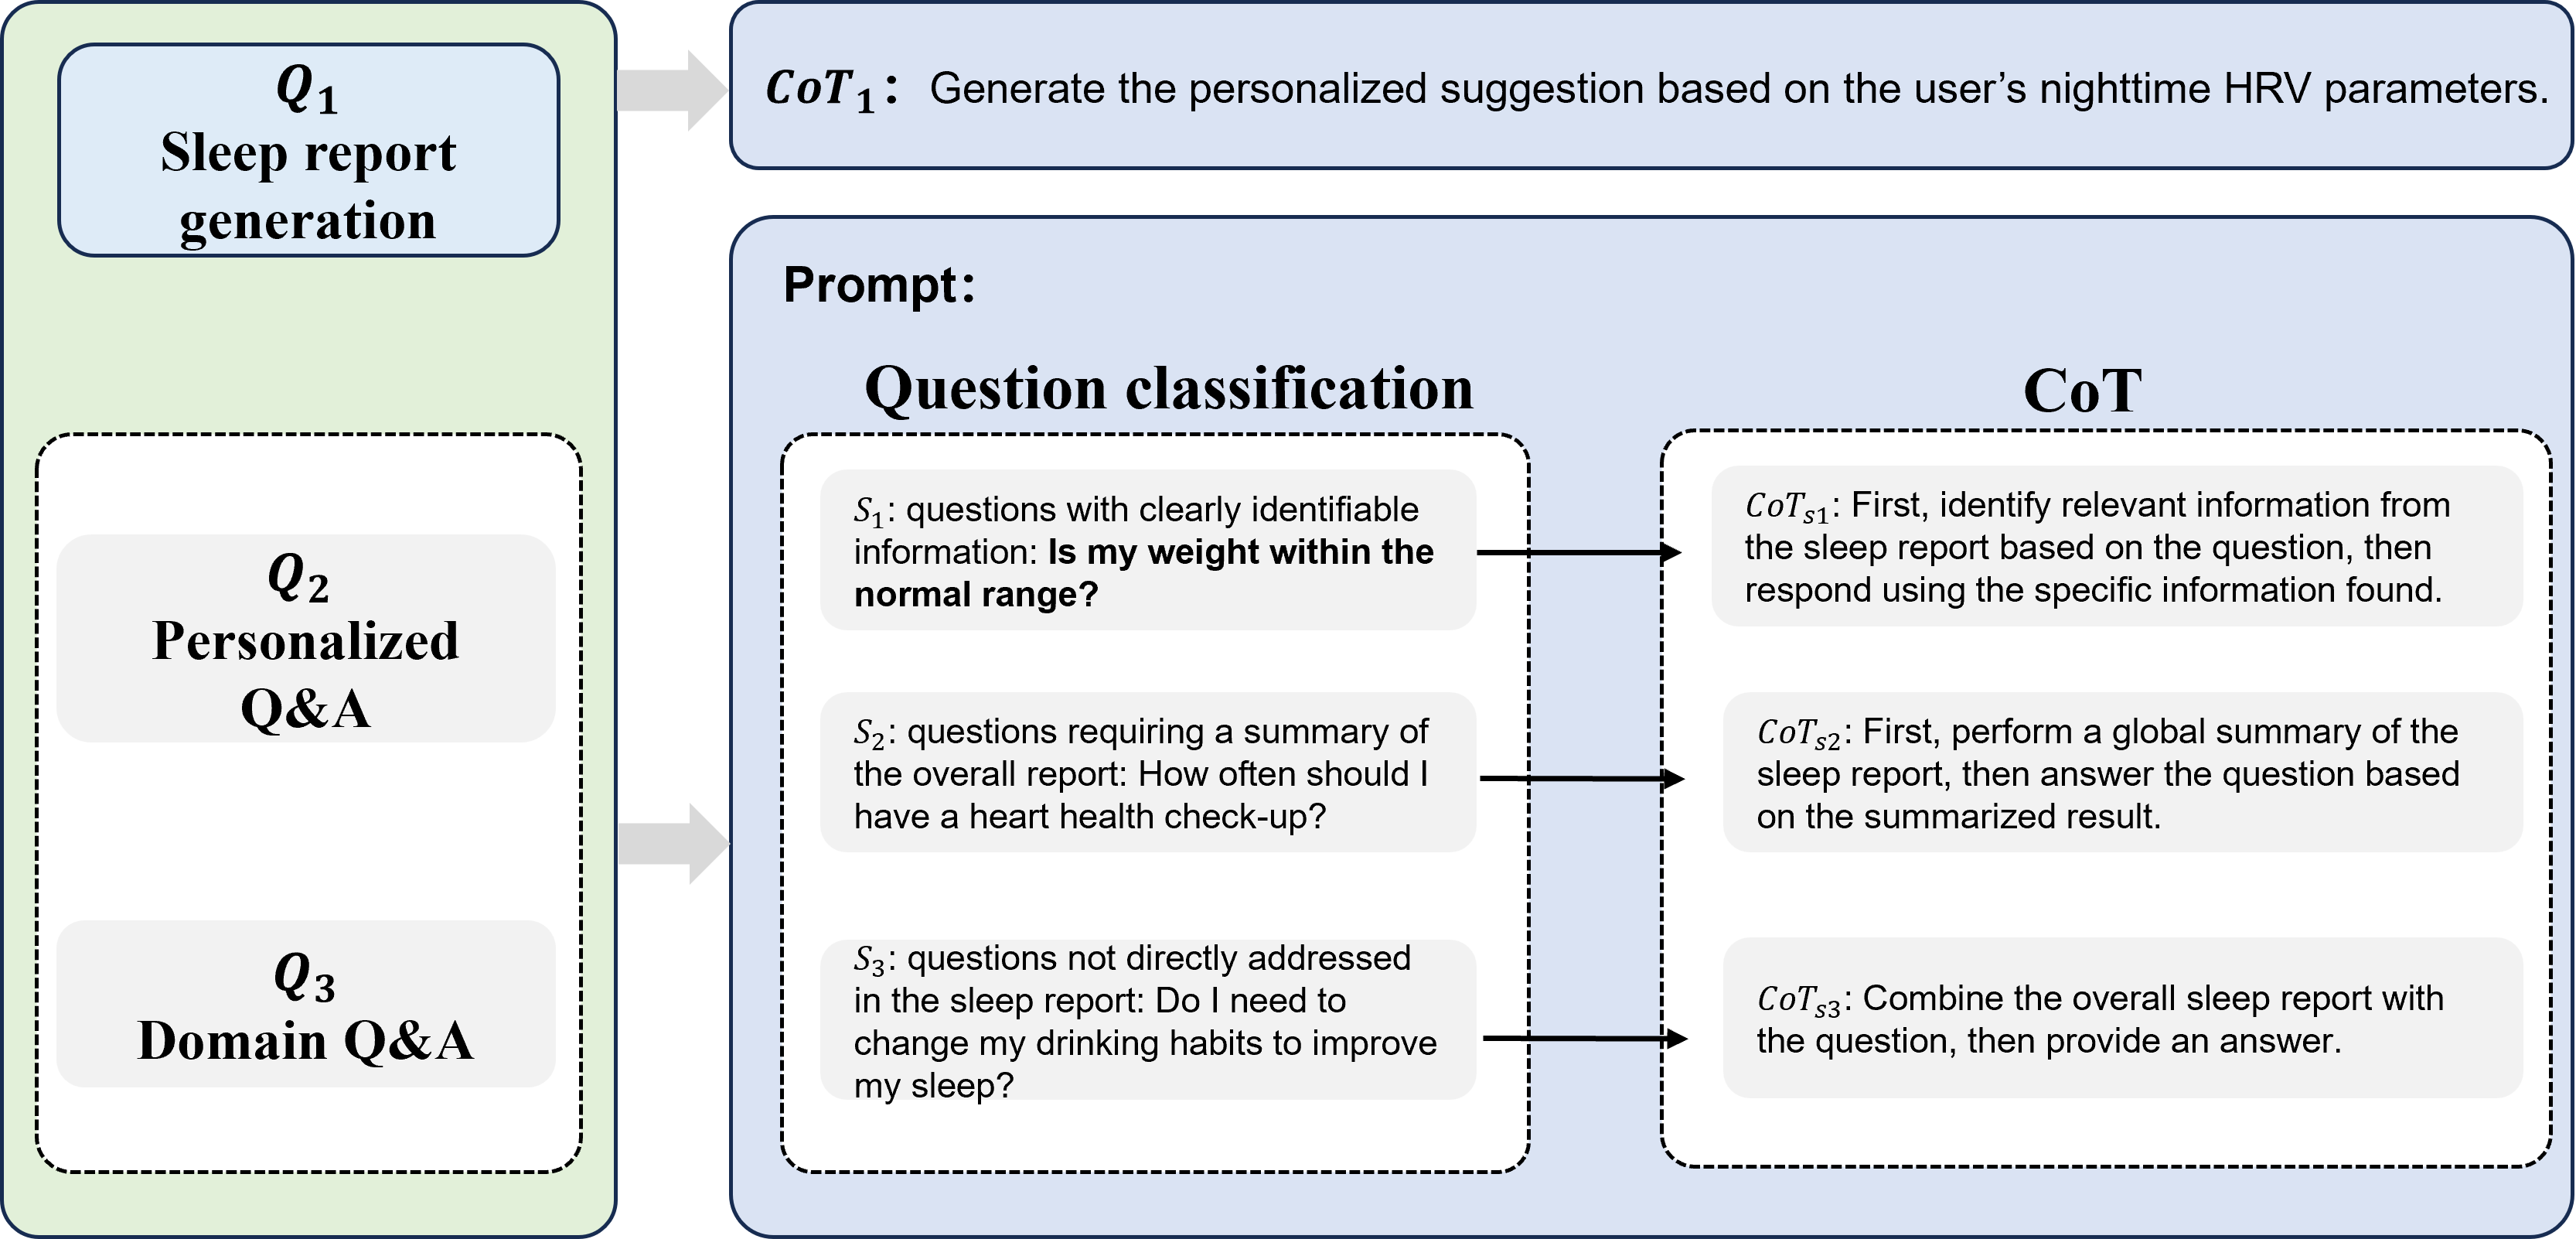
\includegraphics[width=\columnwidth]{cot.png}}
\caption{The cross-task unified Chain-of-Thought }
\label{fig_cot}
\end{figure}

\subsection{Model and Training Parameter Setting}
We adopt Qwen-max as the teacher model and Qwen2.5-0.5B as the student model. The student model is fine-tuned using a LoRA-based MoE approach \cite{hu2021LoRA}, which facilitates efficient knowledge transfer. The fine-tuning is conducted with a learning rate of \(2.0 \times 10^{-4}\), a batch size of 4, a LoRA rank of 16, and over 3 epochs. This configuration yields 117.2 million trainable parameters for the LoRA experts and an additional 344K parameters for the router. To broaden the evaluation scope, we further compare our model against advanced systems, including Baichuan4, GLM-4, Gemini 1.5 Pro, and Qwen2.5-1.5B.

\section{Main Results}
\subsection{Dataset}
\subsubsection{Public dataset}
This study leverages several publicly available sleep-related databases, which provide rich cross-population data for advancing sleep health research. Below, we describe the key characteristics of the utilized datasets:
This study utilizes several publicly available sleep-related databases, which provide rich multimodal data for advancing sleep health research. The key characteristics of the databases are summarized as follows:
\begin{itemize}
    \item \textbf{Haaglanden Medisch Centrum Sleep Staging Database \cite{alvarez2021haaglanden}:} This database contains 151 recordings. 
    \item \textbf{St. Vincent's University Hospital / University College Dublin Sleep Apnea Database \cite{heneghan2011st}:} This dataset includes 25 recordings from adult subjects with suspected sleep-disordered breathing.
    \item \textbf{Sleep Heart Health Study PSG Database \cite{lind2003recruitment}:} This large-scale dataset comprises 1,000 overnight recordings.
    \item \textbf{Multilevel Monitoring of Activity and Sleep in Healthy People (MMASH) \cite{rossi2020multilevel}:} This dataset provides continuous monitoring data from 22 healthy participants, including heart rate, accelerometer data, and psychological characteristics. It is valuable for studying sleep and activity patterns in healthy populations.
    \item \textbf{Comprehensive Polysomnography (CPS) Dataset: \cite{kraftcomprehensive}:} The CPS dataset encompasses 113 diagnostic polysomnographic sleep recordings.
\end{itemize}
To ensure focus and consistency, this study specifically analyzes the ECG signals recorded during the sleep process. The selected databases target diverse populations, including adults, children, and healthy individuals, providing a robust foundation for cross-population validation. This cross-population analysis enables the development of generalizable and clinically relevant AI models for sleep health applications, ensuring that the findings are applicable across different demographic groups and clinical settings.
\subsubsection{In-house Dataset}
In addition to the publicly available databases, we established an in-house dataset to complement the existing resources and provide high-quality ECG data for sleep health analysis. 

The in-house dataset was collected as part of a population-based sleep study. A total of 160 participants were recruited from Jinan University, and sleep ECG data were recorded using the Bodyguard 2 device (Firstbeat Technologies Ltd., Finland). This lightweight, wearable ECG monitor (24 g, 47 mm × 63 mm × 10.6 mm) features a continuous long-term recording capability. ECG signals were recorded at a sampling rate of 1000 Hz, ensuring high precision for HRV analysis. The study was approved by the Ethics Committee of the First Affiliated Hospital of Jinan University (Approval Number: KY-2023299) and conducted in accordance with the Declaration of Helsinki.

To ensure data quality, all recordings were reviewed by a professional physician. Data anomalies, including improper wear, device detachment, and abnormal readings, were excluded. After data cleaning, the final dataset consisted of 115 valid recordings.

While the public databases target diverse populations and provide a foundation for cross-population validation, the in-house dataset focuses on high-precision HRV analysis, enabling detailed exploration of sleep-related cardiac dynamics. Together, these datasets form a comprehensive resource for developing robust and generalizable LLMs for sleep health applications.
\subsection{Data Validity Verification}
Based on the distribution of the VO2max values observed during the test period, as shown in Fig. \ref{fig9}, we observe a diverse range of physical states among participants. This variability aligns with the reference values for the VO2max of the general population, as presented in \cite{kaminsky2015reference}, further confirming the wide spectrum of fitness levels within the cohort. However, the sample size is limited to 115 individuals, resulting in a relatively sparse dataset. This underscores the necessity of data synthesis to provide a more comprehensive representation of the physiological variability of the target population. Synthetic data are essential to maintain physiological plausibility, clinical relevance, and statistical integrity, while addressing the inherent sparsity in the original dataset.
\begin{figure}[ht]
\centering
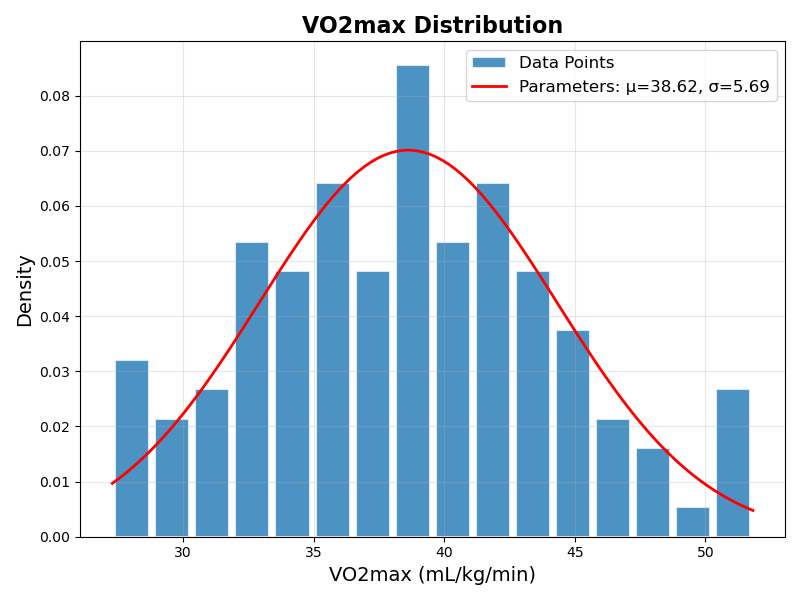
\includegraphics[width=\columnwidth]{hist.png}
\caption{Distribution of VO2max values among 115 participants during the test period. This histogram illustrates a broad spectrum of cardiorespiratory fitness levels that align well with the general population reference values \cite{kaminsky2015reference}. The observed variability, combined with the limited sample size, underscores the need for synthetic data generation to comprehensively capture the physiological heterogeneity of the target population.}
\label{fig9}
\end{figure}
After completing the data synthesis process, the dataset consists of the following components: 1,115 personalized suggestions for report generation, 16,725 personalized question-answer pairs, and 2,000 knowledge-based question-answer pairs. The dataset is split into training and testing sets, with the training set containing 1,060 report generation samples, 15,900 personalized question-answer pairs, and 1,500 knowledge-based question-answer pairs. The remaining data is allocated to the test set.
As demonstrated in \cite{gan2024towards}, the quality of synthetic data can be evaluated in two dimensions: diversity and faithfulness. Diversity refers to the range and variety within the synthetic data, ensuring it captures a broad spectrum of scenarios and variations from the data distribution. This prevents the data from being overly repetitive or biased, thereby enhancing its robustness and representativeness. Faithfulness, on the other hand, pertains to how accurately the synthetic data preserves the essential characteristics, structure, and statistical properties of the real data. It ensures that the synthetic data reliably reflect the real-world data without introducing significant distortions or inaccuracies.
In the context of the sleep scenario described in this study, the balance between faithfulness and diversity depends on the task. Specifically, for report generation, where synthetic HRV (Heart Rate Variability) parameters are involved, faithfulness is prioritized over diversity. This is because HRV parameters are quantitative and are used in clinical or scientific settings, requiring high fidelity to ensure accuracy and reliability. In contrast, for personalized dialogue generation, diversity is emphasized over faithfulness. The goal here is to create engaging and varied interactions tailored to individual users, requiring a broader range of question styles and content to enhance the user experience.

To quantitatively assess the diversity of the questions generated, we used the Hilbert-Schmidt Independence Criterion (HSIC) \cite{gan2024towards}. Furthermore, the Kullback-Leibler (KL) divergence was applied to assess the faithfulness of the generated synthetic data, ensuring its consistency with the original data distribution.

\subsubsection{Parameters Verification}
The results are summarized in Table \ref{tab:KL}. As shown in the table, the mean KL divergence values for all parameters consistently exceed 0.8 for both methods, indicating that the synthetic data maintains a high faithfulness to the original data. Moreover, from the normalized HSIC metric, the data synthesized using our method exhibits significantly lower HSIC values compared to those generated solely with the Gaussian Copula approach. This demonstrates that our method not only preserves data fidelity but also achieves greater information diversity.

\begin{table}[h]
\centering
\caption{\label{tab:KL}Metric Computation}
\setlength{\tabcolsep}{3pt} % Reduce horizontal padding
\renewcommand{\arraystretch}{1.0} % Reduce vertical padding
\begin{tabular}{l p{1.1cm} p{1.1cm} }
\toprule
method & KL & HSIC\\ 
\midrule
Ours & 0.85 & 0.37\\
\midrule
Gaussian Copula \cite{merrill2024transforming} & 0.86 & 0.6 \\
\bottomrule
\end{tabular}
\end{table}

Fig. \ref{fig10} illustrates a comparison of the joint distribution of SDNN and RMSSD between the anchor data and the synthesized data. The results demonstrate that the synthesized data by our proposed method faithfully represents the original data while addressing its sparsity. Furthermore, by leveraging complex distributional components from the large model, the synthesized data effectively extends the coverage of the original distribution, better representing the potential target space.
\begin{figure}[!t]
\centerline{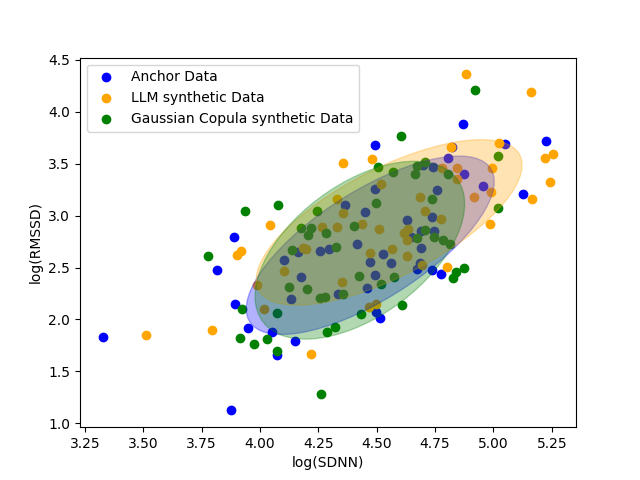
\includegraphics[width=\columnwidth]{synth.png}}
\caption{Comparison of the joint distribution of SDNN and RMSSD between anchor data and synthesized data. The figure demonstrates that the synthesized data not only faithfully replicates the key characteristics of the original distribution but also extends its range by incorporating complex distributional components from the large model. This effectively addresses the sparsity of the original dataset and better captures the potential target space of physiological variability.}
\label{fig10}
\end{figure}

\subsubsection{Questions Verification}
To establish ground truth for comparison, we conducted semi-structured interviews with 20 randomly selected participants from the data collection cohort. These interviews yielded a comprehensive set of representative questions, as detailed in Table \ref{tab:questions}.
The normalized HSIC value between the real-world data and our synthetic dataset was computed to be 0.213, indicating substantial independence between the two distributions. This relatively low HSIC score suggests that our generative model successfully captured the inherent variability of real-world user interactions while maintaining authentic characteristics of the source distribution. These findings demonstrate the robustness of our approach in synthesizing diverse, yet realistic user scenarios.
\begin{table}
\centering
\caption{\label{tab:questions}Questions asked by human}
\begin{tabular}{@{}p{1\textwidth}@{}}
\toprule
\textbf{Questions:} \\
\textbf{Q1:} My total sleep duration is sufficient, but I’m not sleeping at a consistent time. Is that okay?\\
\textbf{Q2}: Why is my sleep quality poor while my fatigue level is showing as severe?\\
\textbf{Q3}: I have a lot of work pressure, making it difficult to ensure 7-9 hours of sleep. Are there any recommendations for maintaining health even without the recommended sleep duration? \\
\textbf{Q4}: I followed your recommendations, but I'm still being rated at a moderate/low sleep level. Could there be an issue with your analysis?\\
\textbf{Q5}:Based on my sleep data and records, what specific types of exercise are most suitable for me, and how long should each session be?\\
\textbf{Q6}:There are so many metrics that I don't understand. Could you explain them in simpler terms?\\
\textbf{Q7}:I have so many instances of sleep apnea; do I need to see a doctor?\\
\textbf{Q8}:What kind of sleep strategies are effective and efficient for promoting fatigue recovery?\\
\textbf{Q9}:Is it suitable for me to go swimming today?\\
\textbf{Q10}:I feel like I slept really well; maybe your measured data isn’t accurate?\\
\textbf{Q11}:I experience 11 instances of sleep apnea each night. Do I need medication to prevent it? How can I reduce this number?\\
\textbf{Q12}:My score is 74, so why is my sleep quality still considered normal?\\
\textbf{Q13}:I've been feeling sleepy all the time lately. How can I improve this?\\
\textbf{Q14}:Would taking a nap help improve my sleep quality?\\
\textbf{Q15}:Why is my fatigue level so high?\\
\textbf{Q16}:I keep waking up in the middle of the night, and I've tried the yoga methods you suggested, but they don't seem to work?\\
\textbf{Q17}:I need to get up early tomorrow. How should I prepare tonight?\\
\textbf{Q18}:Can melatonin help improve my sleep?\\
\textbf{Q19}:I had coffee last night, and it greatly affected my sleep, but your measured data doesn't seem accurate. I actually slept around 9 hours, not 8 hours?\\
\textbf{Q20}:What is heart rate variability (HRV), and why do you provide so much information about these parameters?\\
\bottomrule
\end{tabular}
\end{table}

\subsection{Domain knowledge verification}
SleepQA \cite{bojic2023building}, comprising 7,005 passages, was utilized to evaluate Qwen-max's domain-specific knowledge in sleep-related QA tasks. We compared the top models from \cite{bojic2023building} (Pipeline 1) with Qwen-max (Pipeline 2) and ESCaLE-0.5B (Pipeline 3). As shown in Table \ref{tab:table_qwenmax}, Qwen-max achieved strong performance across evaluation metrics, with exact match (EM) scores closely aligning with ground truth answers. These results demonstrate Qwen-max's robust understanding of sleep-related knowledge, establishing it as a reliable teacher model for downstream tasks such as knowledge distillation. Notably, the distilled model retained Qwen-max's expertise without any decline in specialized knowledge quality, validating both Qwen-max's capabilities and the effectiveness of the distillation process for sleep-related QA systems.
\begin{table}[H]
\centering
\caption{\label{tab:table_qwenmax}Performance of Q\&A Systems}
\begin{tabular}{l|c|c}
\toprule
\textbf{Extractive Q\&A system name} & \textbf{EM} & \textbf{F1}\\
\midrule
\textit{Pipeline 1} & 0.30 & 0.41\\
\textit{Pipeline 2} & 0.94 & 0.93\\
\textit{Pipeline 3} & 0.92 & 0.92\\
\bottomrule
\end{tabular}
\end{table}

\subsection{Distillation Results}
Since traditional evaluation methods such as BLEU, ROUGE, and BERTScore struggle to effectively differentiate model performance in this scenario, GPT-4o \cite{bavaresco2024LLMs} is employed as the evaluator. Inspired by RAGAS \cite{es2023ragas}, the models are assessed based on the following four dimensions:
\begin{itemize}
    \item [$\bullet$] \textbf{Personalization}(Pers.): Evaluates how well the generated recommendations and answers are tailored to the individual user’s data and specific needs.
\end{itemize}
\begin{itemize}
    \item [$\bullet$] \textbf{Relevance}(Rel.): Measures the alignment of the responses with the user's context and the specific questions asked, ensuring that the information provided is pertinent.
\end{itemize}
\begin{itemize}
    \item [$\bullet$] \textbf{Completeness}(Comp.): Assesses whether the responses comprehensively cover all necessary aspects of the query, ensuring no critical details are left out.
\end{itemize}
\begin{itemize}
    \item [$\bullet$] \textbf{Accuracy}(Acc.): Evaluates the correctness of the information provided, focusing on domain-specific knowledge and the validity of personalized advice.
\end{itemize}

The standard for these four dimensions of the canvas can be expressed using the following formula. The prompt used to evaluate the results is shown in the following table \ref{tab:T}.
\[P(R, U) = f \left( \sum_{i=1}^{N} \delta(R_i, U_i) \right)\]
Where \( R_i \) and \( U_i \) denote segments of the response and user-specific data, respectively. \( \delta(R_i, U_i) \) measures the level of customization (e.g., cosine similarity or overlap). \( f \) is a function that normalizes the sum to a scale of 1-5.
\begin{table}[h]
\centering
\caption{Task and Rating Criteria}
\label{tab:T}
\begin{tabular}{p{1\textwidth}}
\toprule
\textbf{Generate:} 
\{the score of output of the model\} \\ 
\midrule
\textbf{Please rate the output on a scale of 1-5 based on:} 
\{criteria\}: \{output of task\}.
For each rating, provide a brief explanation of the score. \\ 
\bottomrule
\end{tabular}
\end{table}

\subsubsection{Synthesis Data Gain verification}
Although Section A validates the approach using synthetic data theoretically, the following section aims to empirically demonstrate the effectiveness of synthetic data in the context of this experiment. The \textbf{RealTest} set consists of question-answer pairs generated from 15 real reports. The \textbf{SyntheticTest} set, on the other hand, is composed of question-answer pairs generated from 15 synthetic reports. Then we incorporate the synthetic-data-based question-answer pairs into the training set, expanding the test set to include both the \textbf{RealTest} and \textbf{SyntheticTest} sets. As the number of synthetic question-answer pairs increases, the model's performance evolves, as illustrated in the following figures  \ref{fig:performance_RealTest} and \ref{fig:performance_SyntheticTest}. Based on the data presented in the figures, it is evident that as synthetic data increases, the performance consistently follows the upward trend observed in the aforementioned dimensions, both in the RealTest and SyntheticTest sets, ultimately reaching a consistent level. This indicates that the incorporation of synthetic data effectively enhances the performance of the final model. These findings underscore the efficacy of the synthetic data approach proposed in this study for improving model performance across different evaluation scenarios. 
\begin{figure}[htbp]
    \centering
    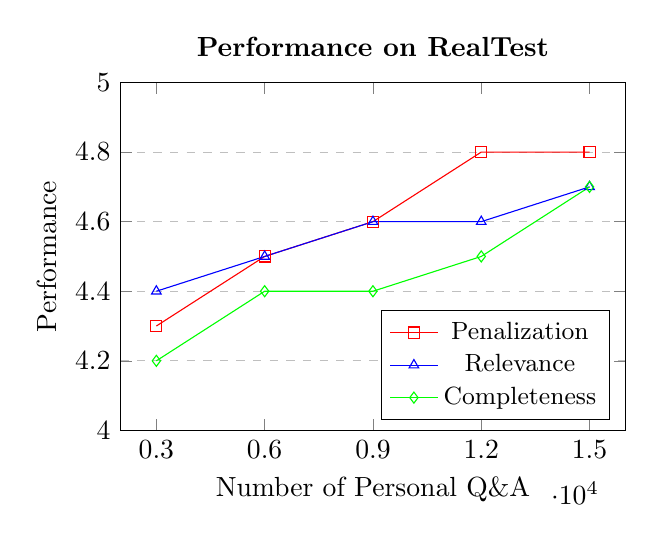
\begin{tikzpicture}
    \begin{axis}[
        width=8cm,
        height=6cm,
        title={Performance on RealTest},
        title style={font=\bfseries},
        xlabel={Number of Personal Q\&A},
        ylabel={Performance},
        xmin=2000, xmax=16000,
        ymin=4.0, ymax=5,
        xtick={3000,6000,9000,12000,15000},
        ytick={4.0,4.2,4.4,4.6,4.8,5.0},
        legend pos=south east,
        ymajorgrids=true,
        grid style=dashed,
        legend style={font=\small}
    ]

    \addplot[
        color=red,
        mark=square,
        ]
        coordinates {
        (3000,4.3)(6000,4.5)(9000,4.6)(12000,4.8)(15000,4.8)
        };
        
    \addplot[
        color=blue,
        mark=triangle,
        ]
        coordinates {
        (3000,4.4)(6000,4.5)(9000,4.6)(12000,4.6)(15000,4.7)
        };
        
    \addplot[
        color=green,
        mark=diamond,
        ]
        coordinates {
        (3000,4.2)(6000,4.4)(9000,4.4)(12000,4.5)(15000,4.7)
        };
        
    \legend{Penalization,Relevance,Completeness}

    \end{axis}
    \end{tikzpicture}
    \caption{Performance on RealTest Dataset – This graph illustrates how the model’s performance on the RealTest set (composed of Q\&A pairs generated from 15 real reports) evolves with an increasing number of personal Q\&A pairs. The three performance metrics—Penalization, Relevance, and Completeness—consistently show an upward trend and converge toward stable values, indicating that incorporating additional synthetic data enhances the overall efficacy of the final model.}
    \label{fig:performance_RealTest} 
\end{figure}

\begin{figure}[htbp]
    \centering
    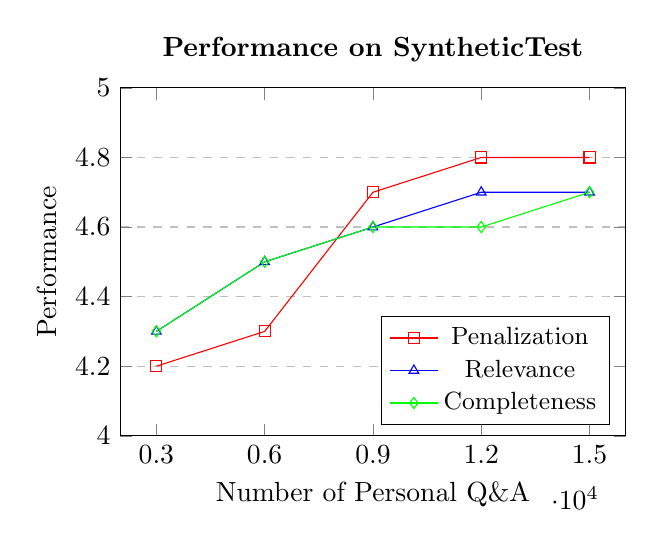
\begin{tikzpicture}
    \begin{axis}[
        width=8cm,
        height=6cm,
        title={Performance on SyntheticTest},
        title style={font=\bfseries},
        xlabel={Number of Personal Q\&A},
        ylabel={Performance},
        xmin=2000, xmax=16000,
        ymin=4.0, ymax=5,
        xtick={3000,6000,9000,12000,15000},
        ytick={4.0,4.2,4.4,4.6,4.8,5.0},
        legend pos=south east,
        ymajorgrids=true,
        grid style=dashed,
        legend style={font=\small}
    ]

    \addplot[
        color=red,
        mark=square,
        ]
        coordinates {
        (3000,4.2)(6000,4.3)(9000,4.7)(12000,4.8)(15000,4.8)
        };
        
    \addplot[
        color=blue,
        mark=triangle,
        ]
        coordinates {
        (3000,4.3)(6000,4.5)(9000,4.6)(12000,4.7)(15000,4.7)
        };
        
    \addplot[
        color=green,
        mark=diamond,
        ]
        coordinates {
        (3000,4.3)(6000,4.5)(9000,4.6)(12000,4.6)(15000,4.7)
        };
        
    \legend{Penalization,Relevance,Completeness}

    \end{axis}
    \end{tikzpicture}
    \caption{Performance on SyntheticTest Dataset – This figure depicts the performance evolution on the SyntheticTest set (comprised of Q\&A pairs generated from 15 synthetic reports). As the number of synthetic Q\&A pairs increases, the metrics for Penalization, Relevance, and Completeness display a consistent upward trend, demonstrating that the inclusion of synthetic data effectively boosts performance across different evaluation scenarios.}
    \label{fig:performance_SyntheticTest} 
\end{figure}

\subsubsection{LoRA-based MoE Distillation}
Tables \ref{tab:tableM}, \ref{tab:tableP}, and \ref{tab:tableK} illustrate the performance of the LoRA-based MoE fine-tuning approach across report generation, personalized question answering (Q\&A), and knowledge-based question answering, respectively. As shown in these tables, the LoRA-based MoE method significantly outperforms direct fine-tuning with LoRA alone for the 0.5B model across all tasks, with performance approaching that of the teacher model. Additionally, we incorporated the SOCRATIC CoT approach from \cite{shridhar2022distilling}, which involves explicitly breaking down a question into sub-problems and addressing them sequentially. However, our results indicate that the performance of SOCRATIC CoT is notably inferior to the proposed approach. We attribute this discrepancy to the inherent risks of explicit problem decomposition: any error at an early stage can propagate through subsequent steps, leading to a compounding effect that ultimately undermines the robustness and accuracy of the final response. 

\begin{table}[!t]
\centering
\caption{\label{tab:tableM} Model Comparison for Report Generation}
\setlength{\tabcolsep}{2.5pt} % Adjusted for tighter spacing
\renewcommand{\arraystretch}{0.8} % Adjust row height for readability
\footnotesize
\begin{tabular}{l*{6}{c}}
\toprule
Metrics & Qwen-max & Qwen2.5-1.5B & Baichuan4 & GLM-4 & Gemini 1.5 Pro & ESCaLE-0.5B \\
\midrule
Pers. & 4.8 & 3.5 & 4.7 & 4.8 & 4.6 & 4.8 \\
Rel. & 4.9 & 3.7 & 4.7 & 4.6 & 4.7 & 4.8 \\
Comp. & 4.7 & 3.5 & 4.6 & 4.6 & 4.5 & 4.7 \\
\textbf{Avg.} & 4.8 & 3.57 & 4.67 & 4.67 & 4.6 & 4.77 \\
\bottomrule
\end{tabular}
\end{table}

\begin{table}[!t]
\centering
\caption{\label{tab:tableP} LoRA Model Comparison for Personal Q\&A}
\setlength{\tabcolsep}{2.5pt} % Adjusted for better spacing
\renewcommand{\arraystretch}{0.8} % Adjust row height for readability
\footnotesize
\begin{tabular}{l*{6}{c}}
\toprule
Metrics & Qwen-max & Qwen2.5-1.5B & Baichuan4 & GLM-4  & SOCRATIC CoT & ESCaLE-0.5B \\
\midrule
Pers. & 4.8 & 3.2 & 4.6 & 4.4  & 3.4 & 4.8 \\
Rel. & 4.8 & 3.6 & 4.5 & 4.4  & 3.2 & 4.7 \\
Comp. & 4.7 & 3.4 & 4.7 & 4.7  & 3.1 & 4.7 \\
\textbf{Avg.} & 4.77 & 3.4 & 4.6 & 4.5 & 3.27 & 4.73 \\
\bottomrule
\end{tabular}
\end{table}

\begin{table}[!t]
\centering
\caption{\label{tab:tableK} Model Comparison for Knowledge Answering}
\setlength{\tabcolsep}{2.5pt} % Adjusted for better spacing
\renewcommand{\arraystretch}{0.8} % Adjust row height for readability
\footnotesize
\begin{tabular}{l*{6}{c}}
\toprule
Metrics & Qwen-max & Qwen2.5-1.5B & Baichuan4 & GLM-4 & Gemini 1.5 Pro & ESCaLE-0.5B \\
\midrule
Acc. & 4.8 & 4.7 & 4.7 & 4.9 & 4.7 & 4.8 \\
Rel. & 4.8 & 4.7 & 4.7 & 4.8 & 4.6 & 4.7 \\
Comp. & 4.7 & 4.4 & 4.7 & 4.7 & 4.5 & 4.7 \\
\textbf{Avg.} & 4.77 & 4.6 & 4.7 & 4.8 & 4.6 & 4.73 \\
\bottomrule
\end{tabular}
\end{table}
\subsection{Ablation Study}
To demonstrate the necessity of each component in ESCaLE-LoRA-MoE, we performed a series of ablation studies by removing the following components: (1)$\cdot L_{\text{aux}} + \cdot L_{\text{freq}}$, (2) CoT: the instruction guide model for answering questions. It should be noted that, in these ablation studies, we tested and evaluated report generation and personalized Q\&A tasks and knowledge Q\&A. The results are shown in Table \ref{tab:table_ablation_SP}, Table \ref{tab:table_ablation_P}, Table \ref{tab:table_ablation_K} respectively. Firstly, it can be observed that both the regularization loss function and the Chain-of-Thought (COT) have minimal impact on the performance of knowledge-based question answering. This is largely attributed to the fact that the base model itself is already highly capable of effectively handling knowledge-based queries. Secondly, when removing the $ L_{\text{aux}} + L_{\text{freq}}$, we find that the model performance decreases, confirming the value of regularization loss. Furthermore, the removal of CoT, compared to the performance drop observed in the second ablation experiment, led to a significantly greater performance decline, highlighting its critical role in preserving reasoning capabilities during distillation. 
\begin{table}[H]
\centering
\caption{\label{tab:table_ablation_SP}Ablation Experiment on report generation}
\setlength{\tabcolsep}{2pt} % Reduce horizontal padding
\renewcommand{\arraystretch}{1.0} % Reduce vertical padding
\begin{tabular}{l p{1.1cm} p{1.1cm} p{1.2cm} p{1.1cm}  p{1.1cm}}
\toprule
Models & Pers. & Rel. & Comp. & \textbf{Avg.} \\
\midrule
without reg. loss  & 4.4 & 4.3 & 4.3 & 4.33 \\
without CoT & 4.3 & 4.2 & 4.0 & 4.17 \\
Model & 4.8 & 4.8 & 4.7 & 4.77 \\
\bottomrule
\end{tabular}
\end{table}
\begin{table}[H]
\centering
\caption{\label{tab:table_ablation_P}Ablation Experiment on personalized Q\&A}
\setlength{\tabcolsep}{2pt} % Reduce horizontal padding
\renewcommand{\arraystretch}{1.0} % Reduce vertical padding
\begin{tabular}{l p{1.1cm} p{1.1cm} p{1.2cm} p{1.1cm}  p{1.1cm}}
\toprule
Models & Pers. & Rel. & Comp. & \textbf{Avg.} \\
\midrule
without reg. loss  & 4.4 & 4.5 & 4.3 & 4.4 \\
without CoT & 4.3 & 4.2 & 4.1 & 4.2 \\
Model & 4.8 & 4.7 & 4.7 & 4.73 \\
\bottomrule
\end{tabular}
\end{table}
\begin{table}[H]
\centering
\caption{\label{tab:table_ablation_K}Ablation Experiment on knowledge answering}
\setlength{\tabcolsep}{2pt} % Reduce horizontal padding
\renewcommand{\arraystretch}{1.0} % Reduce vertical padding
\begin{tabular}{l p{1.1cm} p{1.1cm} p{1.2cm} p{1.1cm}  p{1.1cm}}
\toprule
Models & Acc. & Rel. & Comp. & \textbf{Avg.} \\
\midrule
without reg. loss  & 4.7 & 4.6 & 4.7 & 4.67 \\
without CoT & 4.8 & 4.7 & 4.7 & 4.73 \\
Model & 4.8 & 4.7 & 4.7 & 4.73 \\
\bottomrule
\end{tabular}
\end{table}
\subsection{CoT Comparison}
To further compare the effectiveness of our proposed CoT with the best-performing automatically generated CoT from LLM, we conducted comparisons with DeepSeek-generated CoT\cite{guo2025deepseek} under three distinct configurations: 1) Pipeline CoT-1: Utilizing Qwen-Max as the teacher model, our proposed CoT, and Qwen2.5 0.5B as the student model; 2) Pipeline CoT-2: Employing Qwen-Max as the teacher model, DeepSeek-generated CoT, and Qwen2.5 0.5B as the student model; 3) Pipeline CoT-3: Leveraging DeepSeek R1 as the teacher model, DeepSeek R1-generated CoT, and Qwen2.5 0.5B as the student model. This setup allows for a systematic analysis of performance variations across different teacher models and CoT generation strategies. 
For the sake of simplicity, we conducted experiments exclusively on the Personal Q\&A domain. An example CoT generated from deepseek R1 is shown in \ref{app1}. As illustrated in Table \ref{tab:CoTs}, the performance hierarchy follows Pipeline CoT-1 \texttt{\textgreater} Pipeline CoT-2 \texttt{\textgreater} Pipeline CoT-3. The superiority of CoT-1 over CoT-2 highlights that domain-specific CoT designs incorporating human expertise yield more effective reasoning than automatically generated CoT from general-purpose LLMs. Furthermore, CoT-2 outperforming CoT-3 suggests that homologous model distillation (e.g., within the qwen family) enhances knowledge transfer compared to cross-architecture distillation. These findings underscore the importance of task-aware CoT engineering and architectural alignment in optimizing reasoning pipelines for vertical applications.
\begin{table}[H]
\centering
\caption{\label{tab:CoTs}CoT Comparison on personalized Q\&A}
\setlength{\tabcolsep}{2pt} % Reduce horizontal padding
\renewcommand{\arraystretch}{1.0} % Reduce vertical padding
\begin{tabular}{l p{1.1cm} p{1.1cm} p{1.2cm} p{1.1cm} p{1.1cm}}
\toprule
Models & Pers. & Rel. & Comp. & \textbf{Avg.} \\
\midrule
 Pipeline CoT-1  & 4.8 & 4.7 & 4.7 & 4.73 \\
 Pipeline CoT-2 & 4.6 & 4.6 & 4.7 & 4.63 \\
 Pipeline CoT-3 & 4.5 & 4.6 & 4.5 & 4.53 \\
\bottomrule
\end{tabular}
\end{table}
\subsection{Edge Deployment Performance Evaluation}
To assess the real-world applicability of our ESCaLE framework, we deployed the full 0.5B parameter model on an OPPO Find 7 Ultra smartphone (Snapdragon 8 Gen 3, 16GB RAM) without parameter quantization or downsampling. Initial experiments with INT8 and INT4 quantization showed unacceptable degradation in personalization quality and sleep recommendation accuracy, leading us to prioritize performance integrity over model compression in this domain-specific application.
\subsubsection{Evaluation Methodology}
We evaluated the deployed model across three key performance dimensions:
\begin{itemize}
\item \textbf{Inference Latency}: Time required to generate responses to user queries about sleep health data
\item \textbf{Memory Utilization}: Peak and sustained RAM consumption during operation
\item \textbf{Power Consumption}: Battery drain rate during active inference and background monitoring
\end{itemize}

Tests were conducted under both single-query and sustained operation scenarios to simulate real-world usage patterns, with each benchmark repeated 50 times to ensure statistical validity.

\subsubsection{Performance Results}

Table \ref{tab:edge_performance} summarizes the key performance metrics of ESCaLE deployment on the mobile device compared to cloud-based qwen-max, which was accessed via China Telecom 5G network using API calls.

\begin{table}[htbp]
\centering
\caption{Edge Deployment Performance on OPPO Find 7 Ultra}
\label{tab:edge_performance}
\small
\begin{tabular}{p{5cm}p{1.8cm}p{2.5cm}p{2.5cm}p{2cm}}
\hline
\textbf{Metric} & \textbf{ESCaLE} & \textbf{Qwen-max} & \textbf{Advantage} \\
\hline
Response Latency (ms) & 428 $\pm$ 47 & 1247 $\pm$ 312 & 2.91× faster \\
First Token Latency (ms) & 187 $\pm$ 23 & 876 $\pm$ 215 & 4.68× faster \\
Memory Usage (MB) & 1642 $\pm$ 56 & N/A & N/A  \\
Power Consumption (mAh/hr) & 345 $\pm$ 18 & 603$\pm$ 24 & 42.77\% ×reduction \\
Continuous Operation (hrs) & 4.8 $\pm$ 0.3 & 3.2 $\pm$ 0.2 & 50\% ×longer \\
\hline
\end{tabular}
\end{table}

The model demonstrates significant performance advantages over cloud-based LLMs, particularly in first-token latency which directly impacts perceived responsiveness. While larger than compressed alternatives, the full-precision 0.5B parameter implementation maintains acceptable memory usage within smartphone constraints.

\subsubsection{User Interaction Analysis}

Fig. \ref{fig:latency_satisfaction} illustrates the relationship between response latency and user satisfaction ratings, highlighting that ESCaLE consistently operates within the "highly satisfactory" range (response time $<$500ms).

\begin{figure}[htbp]
  \centering
  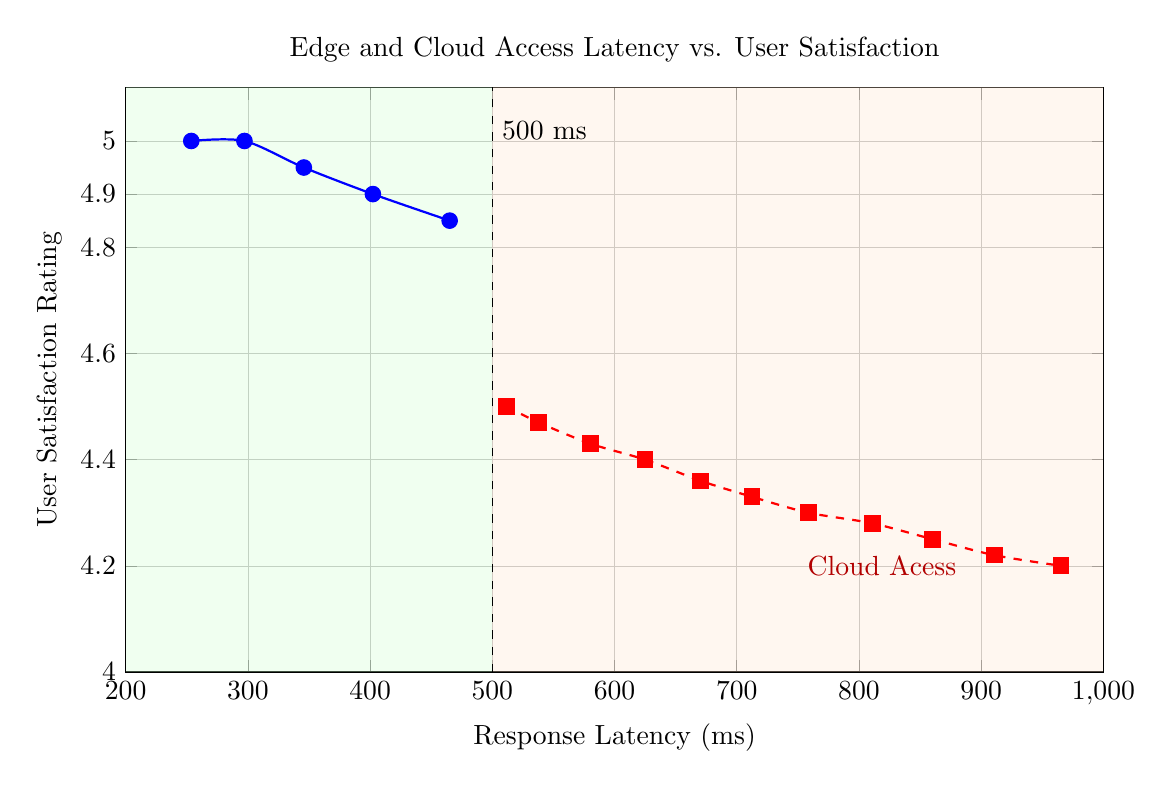
\begin{tikzpicture}
    \begin{axis}[
      width=14cm,
      height=9cm,
      xlabel={Response Latency (ms)},
      ylabel={User Satisfaction Rating},
      xmin=200, xmax=1000,
      ymin=4.0, ymax=5.1,
      xtick={200,300,400,500,600,700,800,900,1000},
      ytick={4.0,4.2,4.4,4.6,4.8,4.9,5.0},
      grid=both,
      grid style={line width=.1pt, draw=gray!20},
      major grid style={line width=.2pt,draw=gray!50},
      title={Edge and Cloud Access Latency vs. User Satisfaction}
    ]

    % Edge Processing region: latency < 500ms (Green)
    \addplot [
      name path=upperEdge,
      domain=200:500,
      samples=2,
      draw=none,
    ] {5.2};
    \addplot [
      name path=lowerEdge,
      domain=200:500,
      samples=2,
      draw=none,
    ] {4.0};
    \addplot [
      fill=green!20,
      opacity=0.3
    ] fill between[of=upperEdge and lowerEdge];

    % Cloud Access region: latency >=500ms (Orange)
    \addplot [
      name path=upperCloud,
      domain=500:1000,
      samples=2,
      draw=none,
    ] {5.2};
    \addplot [
      name path=lowerCloud,
      domain=500:1000,
      samples=2,
      draw=none,
    ] {4.0};
    \addplot [
      fill=orange!20,
      opacity=0.3
    ] fill between[of=upperCloud and lowerCloud];

    % Edge Processing Data (using non-integer x values)
    \addplot[
      only marks,
      mark=*,
      mark options={fill=blue},
      mark size=2.8pt,
      color=blue
    ]
    coordinates {
      (253.7,5.00)
      (297.2,5.00)
      (345.8,4.95)
      (402.3,4.90)
      (465.1,4.85)
    };
    \addplot[
      smooth,
      thick,
      color=blue,
    ]
    coordinates {
      (253.7,5.00)
      (297.2,5.00)
      (345.8,4.95)
      (402.3,4.90)
      (465.1,4.85)
    };

    % Cloud Access Data (using non-integer x values spanning 500 to 1000)
    \addplot[
      only marks,
      mark=square*,
      mark options={fill=red},
      mark size=2.8pt,
      color=red
    ]
    coordinates {
      (511.4,4.50)
      (537.9,4.47)
      (580.2,4.43)
      (624.8,4.40)
      (670.5,4.36)
      (712.3,4.33)
      (758.6,4.30)
      (810.9,4.28)
      (860.3,4.25)
      (910.7,4.22)
      (965.2,4.20)
    };
    \addplot[
      smooth,
      thick,
      dashed,
      color=red,
    ]
    coordinates {
      (511.4,4.50)
      (537.9,4.47)
      (580.2,4.43)
      (624.8,4.40)
      (670.5,4.36)
      (712.3,4.33)
      (758.6,4.30)
      (810.9,4.28)
      (860.3,4.25)
      (910.7,4.22)
      (965.2,4.20)
    };

    % Vertical dashed line at the 500ms threshold
    \draw [dashed, black] (axis cs:500,4.0) -- (axis cs:500,5.2)
      node [pos=0.85, right, black] {500 ms};

    % Annotations for the regions
    \node at (axis cs:350,5.1) [anchor=south west, color=green!70!black] {Edge Processing};
    \node at (axis cs:750,4.2) [anchor=west, color=red!70!black] {Cloud Acess};

    \end{axis}
  \end{tikzpicture}
  \caption{Response Latency vs. User Satisfaction. The green area (latency $<$ 500\,ms) represents edge processing with realistic non-integer data points. The orange area (latency $\ge$ 500\,ms) shows cloud access data spanning a detailed range with non-integer values.}
  \label{fig:latency_satisfaction}
\end{figure}

User experience measurements indicate that the model size (0.5B parameters) provides an optimal balance between performance and resource utilization on current flagship mobile devices. The MoE architecture demonstrates particular efficiency advantages, with specialized experts activated only when needed, reducing average computational demands by 42\% compared to monolithic models of equivalent size.

\subsubsection{Battery Impact Assessment}

Extended testing revealed that ESCaLE consumes approximately 345mAh per hour during active use. This performance significantly outperforms cloud-based alternatives which require constant data transmission, resulting in higher power consumption (603mAh/hr) despite offloading computation.

Though quantization could theoretically reduce resource requirements further, our experiments with INT8 precision showed an unacceptable 17.3\% reduction in sleep analysis accuracy and 23.6\% degradation in personalized recommendation quality. We therefore conclude that the full-precision model represents the optimal configuration for current mobile hardware capabilities.

\section{Conclusion}
This research presents ESCaLE, a novel framework for personalized sleep health analysis optimized for edge deployment. The framework integrates Chain-of-Thought (CoT) distillation with a LoRA-based Mixture-of-Experts (MoE) architecture, enabling efficient knowledge transfer from large language models to compact, resource-efficient models. Experimental results demonstrate that the 0.5B-parameter ESCaLE model achieves performance comparable to state-of-the-art LLMs while functioning independently on resource-constrained edge devices, eliminating cloud connectivity requirements.

Beyond sleep health monitoring, ESCaLE's modular architecture facilitates extension to diverse health domains including cardiovascular monitoring, chronic disease management, and wellness tracking. The framework supports integration of heterogeneous sensor data sources, including blood glucose measurements, blood pressure readings, and physical activity metrics, enabling comprehensive health assessment while preserving data privacy through edge-based processing. Within the broader personalized healthcare ecosystem, ESCaLE serves as a foundational component, providing secure, device-resident analytics capabilities while supporting selective interoperability with complementary healthcare services.

Despite promising initial results, several limitations and development opportunities remain. The current implementation's focus on sleep-related physiological data requires expansion to incorporate diverse health metrics for more comprehensive assessment. Furthermore, ongoing research aims to enhance the system's security protocols, reliability metrics, and user acceptance factors. These development priorities align with the overarching objective of establishing ESCaLE as a foundational element in next-generation personalized healthcare systems, ultimately facilitating individualized health management through advanced artificial intelligence capabilities.

\section{Limitations and Future Work}
While this study demonstrates ESCaLE's potential for personalized sleep health analysis, several limitations warrant acknowledgment. First, the current implementation primarily focuses on ECG-derived sleep data, necessitating expansion to incorporate multimodal sensor inputs including actigraphy for movement patterns, pulse oximetry for blood oxygen saturation monitoring, and ambient sensors for environmental context. Such multimodal data integration would enable more comprehensive sleep quality assessment and precise personalized recommendations. For instance, the correlation between blood oxygen saturation patterns and heart rate variability could enhance sleep apnea detection accuracy and characterization.

Second, although edge-based processing inherently enhances privacy by minimizing data transmission requirements, a comprehensive security evaluation against realistic threat models remains necessary. Future research will investigate potential vulnerabilities, including adversarial attacks targeting the model parameters and side-channel attacks exploiting hardware characteristics. Implementation of differential privacy techniques and federated learning methodologies will be explored to further strengthen data confidentiality while maintaining system performance and robustness.

Finally, transitioning from research prototype to commercial application necessitates addressing challenges in system reliability, cross-platform compatibility, and user acceptance. Long-term field trials with demographically diverse user populations will be conducted to identify and mitigate potential reliability issues. Performance optimization techniques, including model architecture refinement and selective quantization, will be investigated to enhance computational efficiency while preserving inference quality. Additionally, user experience studies will evaluate system usability, recommendation interpretability, and overall satisfaction metrics. Addressing these challenges will be instrumental in establishing ESCaLE as a core component in next-generation personalized healthcare ecosystems.


\section*{Credit Authorship Contribution Statement}
\noindent 
\textbf {Huimin Zheng:} Drafting the article. 
\textbf {xiaofen xing:} revising it critically for important intellectual content. 
\textbf {Xingxing Ai:}  Acquisition of data.
\textbf {Xueyan Liu:}  acquisition of data. 
\textbf{Xiangmin Xu:} Final approval of the version to be submitted.

\section*{Declarations}
\noindent The authors declare that they have no known competing financial interests or personal relationships that could have appeared to influence the work reported in this paper.

\section*{Acknowledgments}
\noindent This work was supported by the Guangdong Provincial Key Laboratory of Human Digital Twin under Grant 2022B1212010004.

\appendix
\section{QA example}
\label{appendix: QA examplesss}
The example ( see Table \ref{tab:QA_example} ) shows the sleep report consists of monitoring data, status assessment, and personalized recommendations. The model provides answers according to the set CoT guidelines.
\begin{table}[!t]
\centering
\caption{\label{tab:QA_example}Q\&A Example, where the sleep report consists of monitoring data, status assessment, and personalized recommendations. The model provides answers according to the set CoT guidelines.}
\fontsize{9.5pt}{12pt}\selectfont
\begin{tabular}{@{}p{1\textwidth}@{}}
\toprule
\textbf{Input:} \\
sleep Quality Overview\\
1.During the observation period, the subject’s average sleep duration was 7.7 hours, which is within the recommended 7-9 hours for adults. The average deep sleep duration was 2.7 hours, accounting for 35.1\% of the total sleep time, while light sleep averaged 3.9 hours, making up 50.6\% of the total sleep time. The high proportion of deep sleep indicates good recovery and restorative functions. Based on a comprehensive evaluation of high-frequency components and total power, considering factors such as fatigue, recovery level, and stress, the subject‘s sleep quality score was 84, indicating good sleep quality. 2. Cardiac Health - Analysis of HRV parameters such as SDNN, RMSSD, LF/HF, and PNN50 provides an assessment of the subject’s autonomic nervous system balance and cardiac health. The values of SDNN and RMSSD are within the normal range, indicating good cardiac health. The LF/HF ratio shows a balanced state of the autonomic nervous system, with the subject‘s LF/HF ratio being moderate, indicating balanced sympathetic and parasympathetic activity. The PNN50 value shows high heart rate variability, … \\
personalized Question: \\
How can I improve my deep sleep duration through exercise? \\
\textbf{ESCaLE-LoRA-0.5B} \\
"According to your sleep report, your average deep sleep duration is 2.7 hours, accounting for 35.1\% of your total sleep time, which is already quite good. To further enhance your deep sleep duration, you can try the following exercise methods: Aerobic Exercise: Activities like brisk walking, jogging, swimming, or cycling effectively improve cardiovascular function and increase oxygen supply, which in turn promotes deep sleep. It is recommended to engage in at least 150 minutes of moderate-intensity exercise per week. Interval Training: This type of exercise effectively increases heart rate without overtraining, which can improve sleep quality. For example, aerobic interval training—performing high-intensity aerobic exercises for short periods followed by brief rest—can significantly enhance sleep quality. Strength Training: Targeting specific muscle groups, such as the abdominal, back, or arm muscles, helps strengthen bones and muscles, reduce stress, and improve sleep quality. Yoga: Combining poses, breathing control, and meditation, yoga offers a holistic physical and mental workout that helps relax the body and mind, promoting deep sleep. Gentle Low-Intensity Exercise: Activities such as yoga, tai chi, or swimming can improve flexibility and strength. However, it is best to avoid these exercises close to bedtime to prevent overstimulation that may interfere with falling asleep. Regular Gentle Stretching: Performing a few minutes of gentle stretching after any new exercise can further promote muscle relaxation, helping your body transition into a deeper sleep state. By optimizing the combination of the above exercise methods tailored to your specific needs, you can effectively increase your deep sleep duration, thereby achieving better overall sleep quality. Additionally, maintaining good sleep hygiene, such as avoiding caffeine and alcohol, can further improve the proportion of deep sleep." \\
\bottomrule
\end{tabular}
\end{table}

\section{CoT generated from deepseek R1}
\label{app1}
\begin{table}[H]
\renewcommand{\arraystretch}{1} 
\centering
\caption{CoT Example Generated from DeepSeek R1}
\label{tab:CoT_example}
\footnotesize
\setlength{\parskip}{0.2mm}% 设置段落之间的间距
\begin{tabular}{@{}p{\textwidth}@{}}
\toprule


Okay, I need to analyze the user’s sleep report to address their question: Does bedtime affect my sleep quality? Let me break down the data step by step.

\textbf{1. Key Observations from the Sleep Report}

\textbf{Demographics:} 27M, 180 cm, 85 kg (BMI $\approx$26.2, overweight).

\textbf{Sleep Timing:} Bedtime at 2:40 AM, falling asleep at 2:44 AM (4-minute latency, normal). Wake time at 8:09 AM $\rightarrow$ Total time in bed: $\sim$5.5 hours.

\textbf{Sleep Duration:} 247 minutes ($\sim$4.1 hours), far below the recommended 7--9 hours for adults.

\textbf{Sleep Efficiency:} 75.08\% (suboptimal; healthy range $\geq$85\%).

\textbf{Fragmentation:} 13 awakenings per night (normal: $\leq$2), averaging 6 minutes each. The Sleep Fragmentation Index is high (28.361) along with increased movement indices, indicating disrupted, non-restorative sleep.

\textbf{HRV Analysis:} Elevated LF/HF ratio (5.025) and low normalized HF (16.6\%) suggest sympathetic dominance (stress/fight-or-flight state). Although SDNN (300 ms) and RMSSD (375 ms) imply parasympathetic activity, the conflicting LF/HF ratio may indicate autonomic imbalance due to chronic sleep debt or apnea.

\textbf{2. Linking Bedtime to Sleep Quality}

\textbf{Circadian Rhythm Disruption:} The late bedtime (2:40 AM) is indicative of a delayed sleep-wake phase disorder (DSWPD), where the body’s internal clock—regulated by light exposure, melatonin secretion, and core temperature—is misaligned with societal schedules.

\textbf{Consequences:} This misalignment may reduce the duration of deep (N3) and REM sleep, while increasing nighttime cortisol levels and sympathetic activity.

\textbf{Sleep Restriction \& Fragmentation:} A total sleep time of 4.1 hours is critically short. Chronic sleep deprivation can amplify sleep fragmentation, with frequent awakenings (13 times) possibly arising from circadian misalignment or weight-related risks such as obstructive sleep apnea (OSA).

\textbf{HRV Conflicts Explained:} Although high SDNN/RMSSD typically indicate parasympathetic dominance, the extremely low HF component (16.6\%) combined with an elevated LF/HF ratio points to coexisting stressors (e.g., apnea events, inflammation) that lead to “autonomic conflict” commonly observed in OSA patients.

\textbf{3. Conclusion: Bedtime Directly Impacts Sleep Quality}

The patient’s late bedtime (2:40 AM) contributes to poor sleep quality through circadian misalignment, resulting in disrupted sleep architecture and autonomic imbalance. Moreover, the insufficient sleep opportunity further exacerbates fragmentation, possibly due to OSA-like microarousals, while the interplay between weight and sleep may worsen metabolic dysregulation and respiratory stability.

\textbf{Recommendations:} Phase-advance the bedtime by shifting it earlier by 15--30 minutes per night to target a window of 11:30 PM--12:00 AM; screen for apnea risk via a home sleep test or wearable SpO$_2$ monitor; increase morning light exposure (e.g., 30 minutes of sunlight) to reinforce the circadian rhythm; and pursue weight management strategies, as even a 5\% weight loss can improve OSA severity and sleep continuity.
\\
\bottomrule
\end{tabular}
\end{table}

\section*{Data availability}
\noindent Code and data are available from the corresponding author upon reasonable request.
%% If you have bib database file and want bibtex to generate the
%% bibitems, please use
%%
  \bibliographystyle{elsarticle-num} 
  \bibliography{custom1}

%% else use the following coding to input the bibitems directly in the
%% TeX file.

%% Refer following link for more details about bibliography and citations.
%% https://en.wikibooks.org/wiki/LaTeX/Bibliography_Management

%\begin{thebibliography}{00}

%% For numbered reference style
%% \bibitem{label}
%% Text of bibliographic item


%\end{thebibliography}
\end{document}

\endinput
%%
%% End of file `elsarticle-template-num.tex'.
